\documentclass[]{iisreport}


% language definition
\lstdefinelanguage[RISC-V]{Assembler}
{
  alsoletter={.}, % allow dots in keywords
  alsodigit={0x}, % hex numbers are numbers too!
  morekeywords=[1]{ % instructions
    lb, lh, lw, lbu, lhu,
    sb, sh, sw,
    sll, slli, srl, srli, sra, srai,
    add, addi, sub, lui, auipc,
    xor, xori, or, ori, and, andi,
    slt, slti, sltu, sltiu,
    beq, bne, blt, bge, bltu, bgeu,
    j, jr, jal, jalr, ret,
    scall, break, nop
  },
  morekeywords=[2]{ % sections of our code and other directives
    .align, .ascii, .asciiz, .byte, .data, .double, .extern,
    .float, .globl, .half, .kdata, .ktext, .set, .space, .text, .word
  },
  morekeywords=[3]{ % registers
    zero, ra, sp, gp, tp, s0, fp,
    t0, t1, t2, t3, t4, t5, t6,
    s1, s2, s3, s4, s5, s6, s7, s8, s9, s10, s11,
    a0, a1, a2, a3, a4, a5, a6, a7,
    ft0, ft1, ft2, ft3, ft4, ft5, ft6, ft7,
    fs0, fs1, fs2, fs3, fs4, fs5, fs6, fs7, fs8, fs9, fs10, fs11,
    fa0, fa1, fa2, fa3, fa4, fa5, fa6, fa7
  },
  morecomment=[l]{;},   % mark ; as line comment start
  morecomment=[l]{\#},  % as well as # (even though it is unconventional)
  morecomment = [s]{/*}{*/},
  morestring=[b]",      % mark " as string start/end
  morestring=[b]'       % also mark ' as string start/end
}

% usage example:

% define some basic colors
\definecolor{mauve}{rgb}{0.58,0,0.82}

\lstset{
  % listings sonderzeichen (for german weirdness)
  literate={ö}{{\"o}}1
           {ä}{{\"a}}1
           {ü}{{\"u}}1,
  basicstyle=\ttfamily,                    % very small code
  breaklines=true,                              % break long lines
  commentstyle=\itshape\color{green!50!black},  % comments are green
  keywordstyle=[1]\color{blue!80!black},        % instructions are blue
  keywordstyle=[2]\color{orange!80!black},      % sections/other directives are orange
  keywordstyle=[3]\color{red!50!black},         % registers are red
  stringstyle=\color{mauve},                    % strings are from the telekom
  identifierstyle=\color{teal},                 % user declared addresses are teal
  frame=l,                                      % black line on the left side of code
  language=[RISC-V]Assembler,                   % all code is RISC-V
  tabsize=4,                                    % indent tabs with 4 spaces
  showstringspaces=false                        % do not replace spaces with weird underlines
}

\usepackage{svg}
\usepackage{tikz}
\usepackage{pgfplots}
\usepackage{pgfplots}


\title{Rust RTOS on ControlPULP}

\author{Noah Zarro}
\email{zarron@student.ethz.ch}
%
\semester{Fall Semester 2022}
% \date{Date of thesis hand-in}
\reporttype{Master Thesis}
%
\professor{Prof. Dr. Luca Benini, lbenini@iis.ee.ethz.ch}
\advisor{Robert Balas, balasr@iis.ee.ethz.ch}
\advisor{Alessandro Ottaviano, aottaviano@iis.ee.ethz.ch}
\advisor{Michael Rogenmoser, michaero@iis.ee.ethz.ch}

\titlelogo{titlepage_logo}
\titlelogoheight{7cm}

\begin{document}

\frontmatter

\chapter*{Abstract}

The abstract summarizes what this report is about.
It focusses on the big picture and does not go into details.
You should write concisely about the following points:

\begin{itemize}
  \item Describe the \textbf{background} of your project: what is the motivation for your project and why is it important?
  \item Describe the \textbf{objectives} of your project.
  \item Describe the \textbf{problems} that must be addressed to achieve the objectives---why are these problems difficult?
  \item Describe your \textbf{approach} and \textbf{methods}.
  \item Summarize the most important \textbf{results}.
  \item State the main \textbf{conclusion} and its significance.
\end{itemize}

The abstract typically takes half a page and should not be longer than one full page.
Try to write a draft of the abstract early on to have a good idea of your project, but revise the abstract as the project progresses.
Write the final version of the abstract once the report is otherwise complete.



\chapter*{Acknowledgments}


Firstly, I would like to thank my supervisors Alessandro Ottaviano, Robert Balas and Michael Rogenmoser who supported me throughout the project. They provided me with technical guidance and also supported me in the planning of the project as a whole.

Furthermore, I have to thank Per Lindgren and his team of the university of Luleå in Sweden, who developed the first version of RTIC, the real time operating system we ported to RISC-V. Without their amazing previous work, this project would not have been possible at all.

And finally, I would like to give my thanks to my friends and family who supported me emotionally through the course of the project.
\chapter*{Declaration of Originality}

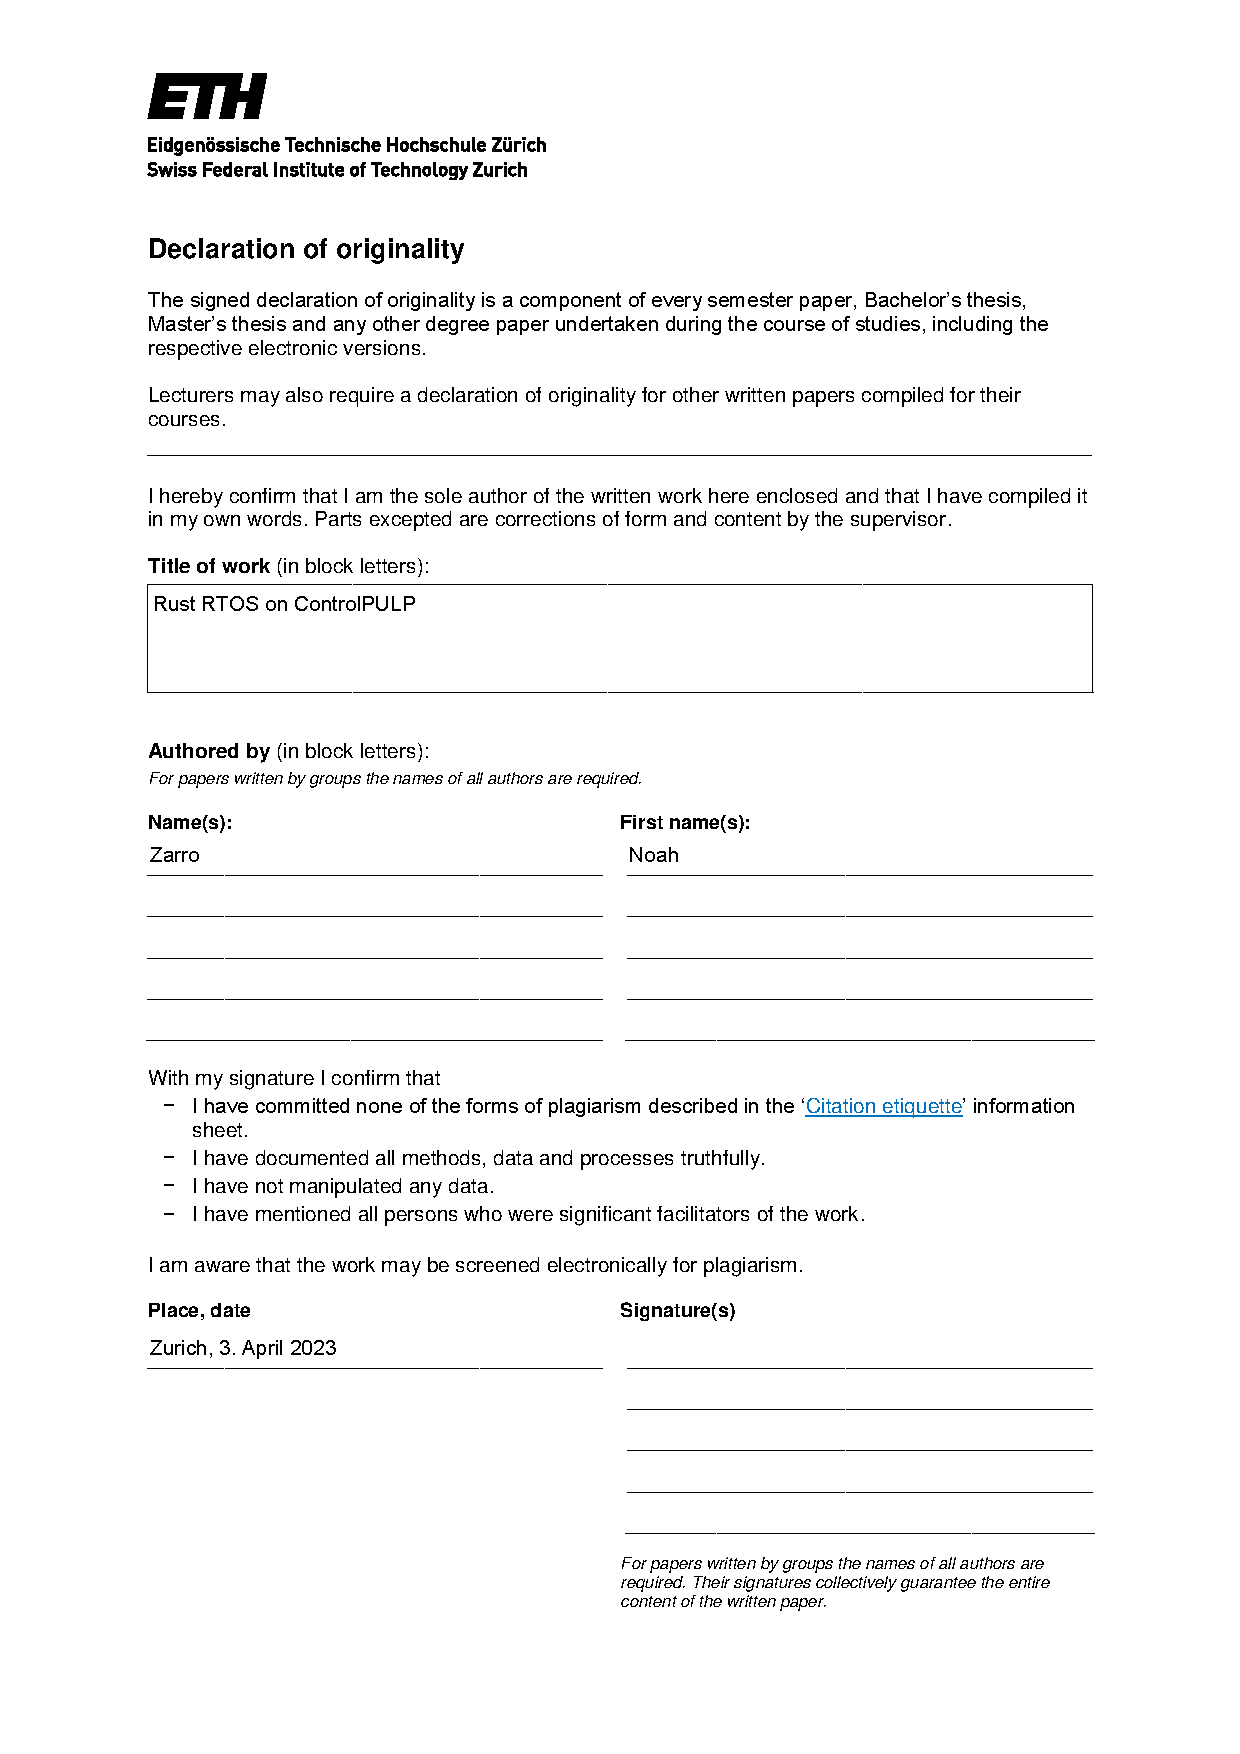
\includepdf[scale=0.9]{declaration-originality-unsigned.pdf}


\tableofcontents

\mainmatter

\chapter{Introduction}
\label{ch:introduction}

The introduction motivates your work and puts it into a bigger context.
It should answer the following questions:
What is the background of this work?
What is the state of the art?
Why is this project necessary to advance the state of the art?
What are the problems that have to be solved and why are they difficult?
What are your contributions to solve these problems?
How do you evaluate your solution to show that it is adequate and applicable?

An introduction written along these questions naturally follows the \textit{\gls{spse}}\footnote{%
  The \acrshort{spse} approach was established in a book~\cite{Hoey83}, but is also briefly summarized in a more recent article~\cite{MP12}, which is available online.
} approach.
In the \emph{situation}, you set the scene for your work and catch the interest of the readers by showing the importance and generality of the scene.
In the \emph{problem}, you spot an issue in the scene and show why and how it significantly taints the scene.
In the \emph{solution}, you outline your solution to that issue.
Finally, in the \emph{evaluation}, you present the main arguments why the claimed solution actually does solve the problem.

In the following chapters, you will elaborate each of the four \gls{spse} elements in detail:
In \textsl{Background}, you lay the foundations for an in-depth understanding of the situation and the problem.
In \textsl{Related Work}, you show how others have address this (or similar) problems and why their solutions are not sufficient or applicable.
In \textsl{Implementation}, you specify your solution, which you then evaluate rigorously for strengths and weaknesses in \textsl{Results}.

At the end of the introduction, you should explicitly show this structure to the reader by briefly explaining how this report is organized.
Instead of using the general \gls{spse} terminology and the chapter names mentioned above, we urge you to use the domain-specific terminology established in the introduction and point to chapters using cross references (e.g., refering to \cref{ch:background} instead of ``the Background chapter'').

\chapter{Background}
\label{ch:background}

Explain the background and theory underlying your project.
Assume that the average reader has the same knowledge you had \emph{before} undergoing this project.
This chapter should transfer all knowledge necessary to understand the following chapters.

As this and the following chapters are likely longer than a few pages, consider structuring them into sections (but avoid fragmentation by overly fine-grained sectioning).
Use the \verb|\..section{}| command family as illustrated below:

\section{RTOS Evaluation}
\label{sec:rtos_evaluation}

Since Rust is a quite new language, there is no dominating open source RTOS yet, as it is the case for FreeRTOS in the Embedded C/C++ world.
Therefore, a few competing RTOS's exist in the Rust embedded world.
The website "Are we RTOS yet?"~\cite{AWRY} lists the most important RTOS's that exist for Rust at the moment.
One criterion for the selection of an operating system was that it is fully written in Rust.
There exist a few RTOS's that are written in C but feature a Rust wrapper.
However, with this setup, the memory safety guarantees by the compiler are lost.
Therefore, we picked six RTOS's with the most stars and forks on GitHub for closer investigation. The chosen OSes were: Bern, Drone, Embassy, Hubris, Tock and RTIC. 

\subsection{Bern}
Bern OS was developed in the process of a master thesis. It features multiple isolated processes, which are scheduled with a preemptive round-robin scheduling algorithm, similar to FreeRTOS. However, since it is a relatively new, one-man project, it was far from sure that it would be continued, therefore we did not choose it~\cite{Bern}.

\subsection{Hubris}
Hubris resembles a more classical OS, since it features a kernel that runs in privileged mode, and tasks that are separately complied and run in an unprivileged mode. However, we preferred a simpler implementation that does not use different privilege modes~\cite{Hubris}. 

\subsection{Tock}
Tock OS was the most popular OS on GitHub, but it turned out that it does not feature prioritized tasks. Since this is essential for an embedded RTOS we did not choose it~\cite{Tock}.

\subsection{Drone/Embassy}
Drone and Embassy both support tasks with different priorities. Tasks with the same priority are cooperatively run using the async/await concept. It would have been an interesting choice, but finally we decided to choose RTIC that was solely based on interrupts, which was also a very interesting concept~\cite{Drone},~\cite{Embassy}.

\subsection{RTIC}
\gls{rtic} is a very light weight operating system that does not feature a kernel or scheduler, but outsources the whole OS-functionality to auto generated interrupt handlers.
It is developed by a team of the university of Luleå in Sweden.
Therefore, long term support seamed likely.
Since it uses the innovative interrupt based task dispatching model, we chose it to port it to the \gls{pulp} platform.

\section{RTIC}
\gls{rtic}, formerly known as RTFM (Real Time For the Masses), provides all features that are needed in an embedded RTOS, while generating minimal overhead.
It features tasks with static priorities. Higher priority tasks can preempt lower priority tasks. Equal priority tasks, however, run sequentially.
There are no message passing queues as for example in FreeRTOS, but tasks can be passed a payload at spawn time.
Furthermore, tasks can access shared resources. However, the list of resources that can be accessed by a specific task has to be given at compile time~\cite{RTIC}. 

\subsection{Code Generation}
Since \gls{rtic} does not feature a kernel, all functionality lies in auto generated interrupt handlers.
The whole \gls{rtic} program has to be defined inside a \texttt{\#app} macro. At compile time, the macro processor performs a static analysis of the program. The number of tasks, their priorities and the resources that can be accessed by the tasks are determined. With this information, a few interrupt handlers are generated. They are described in the following.

\subsubsection{Task Dispatcher}
Task dispatchers are responsible for the execution of all tasks of a specific priority.
They are bound to an interrupt that is configured to the same priority.
Each task dispatcher contains a queue with references to all tasks that are ready to be executed at a specific moment.
If a task is to be spawned, a reference to the task is placed in the ready queue of it's corresponding task dispatcher.
Thereafter, the task dispatcher's interrupt is pended in software. The interrupt handler only consists of a loop through the ready queue.
For each reference to a task in the ready queue, a corresponding task instance is run inside the interrupt handler.
With this system, no scheduling algorithm is needed, since higher priority tasks will always preempt, or in this case interrupt, lower priority tasks.
Same priority tasks run cooperatively.

\subsubsection{Timer Handler}
With task dispatchers, it is only possible to spawn tasks that run immediately.
To spawn tasks in the future, the timer handler is generated. It is an interrupt handler for a timer interrupt.
The timer handler is unique in the system, and handles tasks of all priorities.
The timer interrupt is set to the maximum priority.
If a task spawn is scheduled in the future, a reference to the task is placed in the timer queue of the timer handler, together with its desired spawn time.
As soon as the timer queue is modified, the timer comparison value is adjusted, such that the timer interrupt fires at the spawn time of the task that will start first.
If the timer interrupts and the handler is started, it moves all tasks that are still in the timer queue and became ready into their corresponding task dispatcher, and pends its corresponding interrupt in software.
Since the timer interrupt is running at maximum priority, this happens immediately.
Since the actual running of the tasks is still handled by the task dispatcher, the priorities are still respected.

\subsubsection{Shared Resources}
Since it is known at compile time which tasks will access which resources, the locking of resources can be simplified.
During the evaluation of the \texttt{\#app} macro, for each shared resource, a list is generated with all tasks that could access the resource.
Tasks can only be preempted by other tasks, if a task dispatcher interrupt with higher priority fires.
Therefore, to lock a shared resource, one can just temporarily raise the interrupt level threshold of the system to the highest level of any task that also has access to the shared resource. Like this, it is guaranteed, that no other task can access the shared resource while it is locked.
If a task itself is the one with the highest priority, accessing a specific resource, the locking of this resource is completely optimized out at compile time.

\section{Rust Embedded Ecosystem}

\begin{figure}
  \centerfloat
  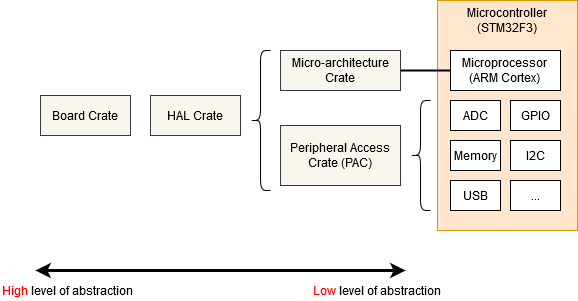
\includegraphics[width=\textwidth]{fig/crates.png}
  % Note: We do not have the SVG source file for the image above, so we have to put the PDF under version control.
  \caption{TODO: Create SVG}%
  \label{fig:embedded_crates}
  % Note: The `\label{}` can be on the line after the `\caption{}` if the `\caption{}` line ends with a comment.
\end{figure}

Since Rust appeared only very recently, the community already gained a lot of experience in embedded development.
Therefore, attempts were made to standardize and categorize embedded libraries.
There are several types of libraries, or crates, as they are called in Rust, see figure \ref{fig:embedded_crates}.
The most of the embedded libraries in Rust are strongly focused on the ARM Cortex-M architecture. Implementations for RISC-V microcontroller did exist, however, they are usually very minimalistic. See section~\ref{sec:libraries} for an overview of the necessary changes for RISC-V.

\subsection{Micro-architecture Crate (MAC)}
These crates handle any useful routines common to the processor core of a specific microcontroller, as well as any peripherals that are common to all microcontrollers that use that particular type of processor core. For example, the cortex-m crate gives features functions to enable and disable interrupts, which are the same for all Cortex-M based microcontrollers. It also gives you access to the 'SysTick' peripheral that is included in all Cortex-M based microcontrollers~\cite{RustEmbedded}. There also exists a very basic crate for RISC-V.

\subsection{Peripheral Access Crate (PAC)}
These crates are thin wrappers for the various memory-wrapper registers defined for a particular part-number of microcontroller. For example, stm32f30x for the ST-Micro STM32F30x series. Here, registers can be accessed directly, following each peripheral's operating instructions given in the microcontroller's Technical Reference Manual~\cite{RustEmbedded}.

\subsection{HAL Crate}
These crates offer a more user-friendly API for a particular processor, often by implementing some common traits defined in embedded \gls{hal}. It therefore makes use of the trait system, that could be compared to interfaces in Java. For example, this crate might offer a Serial struct, with a constructor that takes an appropriate set of GPIO pins and a baud rate, and offers some sort of \texttt{write_byte} function for sending data~\cite{RustEmbedded}. 

\subsection{Board Crate}
These crates go one step further than a \gls{hal} crate by preconfiguring various peripherals and GPIO pins to suit a specific developer kit or board, such as stm32f3-discovery for the STM32F3DISCOVERY board~\cite{RustEmbedded}.

\subsection{Runtime Crate}
These crates provide all code that is required to get to main. They usually feature either some low level Rust or even assembly code that initializes all registers, such as the stack pointer, setup interrupt vectors and finally call \texttt{main}. Furthermore, they provide macros to specify interrupt handlers. A RISC-V version of a runtime crate does exist, however only in a minimalistic version, without interrupt handler support.

\section{Interrupt Controller}
\label{sec:interrupt_controller}
Since \gls{rtic} heavily relies on interrupts for tasks, it is also very dependent on a powerful interrupt controller hardware.
Originally, \gls{rtic} was designed to be used with the \gls{nvic}.
For RISC-V the \gls{clic} is the most advanced interrupt controller available.
Fortunately, they are quite similar.
In the following, their major features are explained, and the main differences are stressed out~\cite{NVIC}\cite{CLIC}. 

\subsection{Vectorization}
\label{sec:vectorization}
The \gls{nvic} and the \gls{clic} are both vectorized interrupt controllers.
For the \gls{nvic}, this means, that there exists a table of addresses of interrupt handler functions, the vector table. For each interrupt, there exists an entry in the table. If an interrupt occurs, the program counter is set automatically to the address of the interrupt handler that is associated with the interrupt.
According to the specification, the vector table of the \gls{clic} works in the same way.
In the specific implementation of our group, however, it is not filled with addresses, but with jump instructions to the different interrupt handlers.
It has the same effect, but requires a different setup process of the interrupt table.~\cite{NVIC}\cite{CLIC}

\subsection{Configuration}
\label{sec:interrupt_configuration}
Both the \gls{nvic} and the \gls{clic} allow for setting priority levels for interrupts individually.
Higher priority interrupts preempt lower priority interrupts.
Both implementation feature 256 interrupt levels. However, while for the \gls{clic} the most urgent interrupt has priority 255, the \gls{nvic} inverts priority levels, and considers interrupts with the lowest priority value as the most urgent.
Similarly, the triggers can be configured for each interrupt individually. Both \gls{clic} and \gls{nvic} feature level and edge sensitive triggers. For certain implementation of \gls{nvic} and all \gls{clic} implementations, it is possible to set priority threshold. Interrupts with priority below this threshold can be pended, but will not be executed until the threshold is lowered. For both implementations, this threshold can be dynamically changed at runtime.
Furthermore, for the \gls{clic}, interrupts can be configured to be non vectorized, and therefore they will use the same handler as the default exception handler. 
~\cite{NVIC}\cite{CLIC}.


\chapter{Implementation}
\label{ch:implementation}

\section{Libraries}
\label{sec:libraries}
Since RISC-V support is minimal in the Rust embedded world, several libraries had to be created or extended.

First, the RISC-V \gls{mac}, had to be extended with support for the \gls{clic}.

Furthermore, in the runtime crate, the vector tables needed to be set up such that they are compatible with the \gls{clic}. Also in the runtime crate, we implemented a macro (the Rust equivalent of a function attribute) to specify interrupt handlers.

Finally, we created a \gls{pac} for the ControlPULP IP, a \gls{rtic} compatible timer wrapper crate and a crate with print support for the QuestaSim simulation.

In the following, the important performed changes and additions to the libraries are explained in detail.

\subsection{Control Status Registers}
The \gls{clic} introduces a variety of new CSRs, that are added to the \gls{mac}. Among others, it includes the \texttt{mintthresh} register, that allows to set the interrupt priority threshold as described in section \ref{sec:interrupt_configuration}. Only the machine mode \gls{csr}s are added to the \gls{mac}, because the test IP only features machine mode. The \gls{csr}s for the other modes could be easily added.

\subsection{Setup}
Since the \gls{clic} calls for a different interrupt configuration procedure at startup than the default RISC-V interrupt controller, the runtime crate was adjusted accordingly.
If an interrupt or an exception occurs, there are two possibilities how it can be handled.
Either, it is a vectorized interrupt that can be handled by an entry in the vector table. The start address of the vector table is then read from the \texttt{mtvec} \gls{csr}. 

On the other hand, if an exception, or a non vectorized interrupt has to be handled, the default handler address is read from the \texttt{mtvt} \gls{csr}.

Therefore, during the startup process, these two registers need to be set accordingly. They are set to the addresses of the labels \texttt{interrupt_vector} and \texttt{_start_trap}. Per default, the \texttt{_start_trap} label is set to a function that just does an infinite loop.

\subsection{Interrupt Vector}
\label{sec:vector_table}
The runtime crate provides a piece of assembly code with jump instructions to the labels \texttt{int_0} to \texttt{int_264}. These labels can be defined by the user in different ways, as described in section \ref{sec:interrupt_handler_macro}.

 This code is linked together with the program and set to be accessible with the label \texttt{interrupt_vector}.

\subsection{Context Switch}
\label{sec:context_switch}
As soon as an interrupt handler is called, a full context switch has to happen. This means that all caller saved registers must be saved to the stack. If nested interrupts are allowed, the \gls{csr}s \texttt{mcause} and \texttt{mepc}, the cause of the interrupt and the return address, have to be saved as well. Furthermore, the callee saved registers must be saved as in any other function.

\subsection{Interrupt Handler Macro}
\label{sec:interrupt_handler_macro}
GCC provides a function attribute \texttt{__attribute__ ((interrupt ("machine")))} that can be added to a RISC-V interrupt handler and handles all necessary steps described in section \ref{sec:context_switch}. For Rust, however, this did not yet exist. Therefore, in the runtime crate, we implemented a procedural macro \texttt{\#[interrupt_handler()]} that generates code that accounts for the context switch.
First, an assembly code block is generated as seen in listing \ref{lst:interruptHandler}.
It performs the context switch. Then it jumps into the actual handler function, that is a normal Rust function. Since it is a normal Rust function, it saves all callee saved registers.
As soon as the handler function returns, the context is restored again.
Ideally, only the callee saved registers that are actually used by the handler function would be saved. However, to achieve this, compiler support would be needed, which is not yet available for Rust. And furthermore, the handler function would have to be a leaf function, which is a strong restriction.

\begin{lstlisting}[language={[RISC-V]Assembler}, caption={Interrupt Handler Wrapper}, label={lst:interruptHandler}]
    .global wrapper_label
    wrapper_label:
    addi sp, sp, -(4 * 32)
    sw ra, 0(sp)
    /* save t0 to a5 (all caller save registers) */
    sw t6, 60(sp)
    csrr t0, mcause
    csrr t1, mepc
    sw t0, 64(sp)
    sw t1, 68(sp)
    csrsi mstatus, 8 /* enable global interrupts*/
    
    jal handler_label /* jump to rust handler function */
    
    csrci mstatus, 8 /* disable global interrupts*/
    lw t0, 64(sp)
    lw t1, 68(sp)
    csrw mcause, t0
    csrw mepc, t1
    lw ra, 0(sp)
    /* restore t0 to a5 (all caller save registers) */
    lw t6, 60(sp)
    addi sp, sp, (4 * 32)
    mret
\end{lstlisting}

\subsection{Labels}
\label{sec:interrupt_macro_labels}
The labels in listing \ref{lst:interruptHandler} are determined as follows. The \texttt{handler_label} is set to \texttt{<handler_name>_handler}, where \texttt{<handler_name>} the name of the original Rust handler function to which the \texttt{\#[interrupt(arg)]} macro is added. The \texttt{wrapper_label} can be set in three different ways, that depend on the argument \texttt{arg} of the macro. If the macro is a number \texttt{i}, then the \texttt{wrapper_label} is set to \texttt{int_i}. It directly corresponds to the label in the vector table, see section~\ref{sec:vector_table}.

Alternatively, the argument can be set to a name of an interrupt enum, defined in the \gls{pac} crate. 
The \gls{pac} crate contains an enum with all interrupts available in this \gls{soc} with meaningful names, as for example \texttt{UART0}. In this scenario, \texttt{wrapper_label} is set to the string representation of the enum identifier.
The linker script in the \gls{soc} crate contains a list of \texttt{PROVIDE(int_23 = UART0);} entries, one for each enum item. Like this, the symbol \texttt{int_i} is set to the address of the corresponding enum label, if \texttt{int_i} is defined nowhere else. This way of assigning interrupts is used by \gls{rtic}

Finally, if the argument is omitted, the \texttt{wrapper_label} is just set to the original name of the handler function (the new name of the handler function is now \texttt{<original_name>_handler}). In this case, the corresponding \texttt{PROVIDE(int_i = <original_name>)} has to be added manually to the linker script of the program.

\section{NXTI}
\label{sec:nxti}
The \gls{clic} contains a hardware extension that can be used to avoid unnecessary context switches. It is a \gls{csr} that provides the address of the vector table entry of the next interrupt that is pending and can be handled in the current context, while no context switch is necessary. The software changes used for nxti support can be activated by using the \texttt{nxti} feature in the runtime and \gls{rtic} crate.

\subsection{Implementation}
To make use of the nxti \gls{csr}, the interrupt procedure must be changed. The vector table is now filled with jump instructions directly to the Rust handler functions. Since by directly jumping to the Rust functions, there would be no context saving or restoring, vectorizing of interrupts is disabled. Therefore, all interrupts are handled by a single interrupt handler, the \texttt{_nxti_trap_handler} that is defined in the runtime crate. It is described in listing \ref{lst:nxtiHandler}.

First, the context is saved. Then a loop is executed that checks if any other interrupt can be handled. Any interrupt that is pending and has greater priority than the saved interrupt context can be served. The available interrupts are then executed sequentially. This means that the processor jumps and links (\texttt{jal}) to the vector table entry of the interrupt that must be served. There it jumps (\texttt{j}) to the Rust handler function and then returns directly back to the \texttt{_nxti_trap_handler}.

If there are no more interrupts that can be served in the current context, the original context is restored, and program execution resumes where the original interrupt happened.

\begin{lstlisting}[language={[RISC-V]Assembler}, caption={Nxti Trap Handler}, label={lst:nxtiHandler}]
.global _nxti_trap_handler
_nxti_trap_handler:
addi sp, sp, -(4 * 32)
/* store context */

/* read out the address of the vector table entry
of the next pending interrupt */
/* a read automatically enables interrupts, and clears
the pending bit of the found interrupt */
1:
csrrsi t0, 0x345, 8

/* if no interrupt is pending, the received addr (t0) will be 0 */
beqz t0, 2f

/* jump to interrupt vector table that contains the
jump instruction pointing to the Rust handler function */
jalr t0

/* repeat until no more interrupts are pending */
j 1b

2:
csrci mstatus, 8 /* disable global interrupts*/

/* restore context */
addi sp, sp, (4 * 32)

/* return to code before initial context save */
mret
\end{lstlisting}

\section{RTIC}
\label{sec:rtic_port}
Since \gls{rtic} was hard-coded to the ARM Cortex-M architecture and therefore the usage of the \gls{nvic}, all references to \gls{nvic} had to be changed to their corresponding \gls{clic} functions. Fortunately, \gls{nvic} and \gls{clic} work quite similar and offer nearly identical functionality. First, we planned to implement functionality to switch between architectures. But this would have meant to introduce a new layer of abstraction. And since \gls{rtic} version 2 was already in development, which should feature a more modular design, we decided not to change version 1 to a modular design but provide our RISC-V insights to the developers for their new version.

However, a few details were not straight forward and will be described in the following.

\subsection{Interrupt Setup}
The setup of the interrupts for \gls{nvic} and \gls{clic} differ, since the \gls{clic} offers more configuration options. For the \gls{clic} vectorization must be enabled for each interrupt if nxti is not used. 

\subsection{Logical Priorities}
\gls{rtic} uses internal logical priorities. Here, 1 is the lowest priority, and 256 is the maximum priority. Since the \gls{nvic} uses inverted priorities as described in section \ref{sec:interrupt_configuration}, a logical to hardware priority conversion function is necessary. The \gls{clic} however uses priorities 0 to 255. So we changed this function to respect the \gls{clic} hardware priority system.

\subsection{Interrupt Handlers}
In the \gls{nvic}, context switching is handled in hardware. Therefore, there is no need for special treatment of interrupt handler functions in Rust. For the \gls{clic} however, special interrupt handler macros are needed, as described in section \ref{sec:interrupt_handler_macro}. We edited the \gls{rtic} code generation to add macros to the generated interrupt handlers.

\section{Toolchain}
With Cargo, Rust provides a straight forward build system. Therefore, we used Cargo to build our test environment. To run the simulation, however, make was used, since the simulation setup was already implemented in Makefiles. Therefore, also the cargo build command is wrapped inside a make command.

\subsection{Build Process}
To build a testing program, \texttt{make all} can be invoked.
It runs \texttt{cargo build ---release}.  If \texttt{nxti=1} is set in the make command, then the nxti feature is used in the runtime and \gls{rtic} crate. If \texttt{no_atomics=1} is set, the program is compiled for a target without atomics.

In the file \texttt{build.rs} all linker scripts are listed that must be used by the linker. The order is important, since symbols that are added to the vector table need to be assigned the correct address. See section \ref{sec:interrupt_macro_labels}.

\subsection{ABI}
As described in section \ref{sec:register_count}, there exist two ABIs and also the E-Extension that change the register count, or the purpose of registers. Such changes need compiler support.
The Rust compiler uses the LLVM framework. However, LLVM does not support any of these additions. Support is currently being added to LLVM~\cite{llvmRISCVEExtension}. We tried to build LLVM from source, with these new extensions included. But it is not possible to configure the Rust compiler to use just any LLVM backend, since it has to be a custom fork of LLVM that adds a lot of changes explicitly for Rust.

Therefore, due to timing constraints, we did not use the E-Extension and the EABI.
\chapter{Results}
\label{ch:results}



\section{Evaluation setup}

\label{sec:comparison_targets}
To evaluate the performance of the \gls{rtic} port to RISC-V, there are two natural options. Either the performance of the OS is compared to another OS that is running on RISC-V. In this case, this would be FreeRTOS, since it is widely used in the group. With this method, one could identify advantages or disadvantages of \gls{rtic}.

The other option is to compare the port of the OS to its original version on its native platform. In this case, this would be \gls{rtic} on ARM Cortex-M. This makes it possible to identify performance differences between the two architectures. This is more interesting for the group, since we mainly work in hardware development and not OS development.

To compare two RTOS implementations, there are again two natural options. One could write a program with a realistic workload, and run it on both setups that should be compared. To identify differences in hardware performance, however, it makes more sense to compare the core transitions of the ROTS on both platforms. With this setup, we can clearly identify where our RISC-V implementation has room for improvement compared to ARM.

\subsection{Platform}
The platforms that are used to perform the measurements were on one side a physical NUCLEO-F103RB evaluation board with a built-in STM32F103RB processor.

On the other side, we use an RTL simulation of the controlPULP IP in QuestaSim. 

\subsection{Time Measurement}
\label{sec:time_measurement}
To measure the time that certain operations take, there are a few options. If an RTL simulation is used, the exact points in time at which an instruction is executed can directly be read out.

Another possibility would be to toggle GPIO pins at certain points in time, and measure the time in between with an oscilloscope. This however only works on a physical device and introduces a lot of measurement uncertainty.

In any other setup, however, it comes down to counting cycles. These can either be counted using a timer that is attached to the main clock. In this case, the timer value can simply be read out. Or it can be counted by reading out the processor's cycle count registers. 

Since counting cycles is the only option that is available on both platforms, it is the best way to acquire measurements that are actually comparable. Therefore, we use the built-in cycle counters for time measurements. On RISC-V they are even a bit more accurate than timer value readouts, since the timer value read needs to load the address of the timer value register into a temporary register, while the cycle counter can be accessed with one single \gls{csr} read.

In actual numbers, this means that for RISC-V the measurement overhead added to the measurement result is between 2 and 3 cycles. \gls{csr} read overhead varies in this range.

For ARM, the overhead cannot be determined exactly, since we do not have access to a cycle accurate simulation. But there are a \texttt{load immediate} and a \texttt{load word} instruction used for the cycle read out. This leads to an estimated overhead of 2 cycles.

For RISC-V the \texttt{mcycle} \gls{csr} is used. For ARM, cycle counts are read from the \texttt{SysTick} counter register.

\subsection{Evaluation Programs}
There exist two standalone programs for RISC-V and ARM that can be run. They measure all core transitions explained in section~\ref{sec:core_transitions}. The output is directly displayed as a print statement.

The setup process and the commands needed to run the programs are described in the README of each program. 

They can be found TODO: insert program links.


\section{Core Transitions}
\label{sec:core_transitions}

We decided to measure core OS transitions for the reasons explained in section \ref{sec:comparison_targets}. In the following, all core transitions that are measured are described. We mainly focus on task spawns, since they are the most important actions in \gls{rtic}. To get an understanding of how the task spawning works in \gls{rtic}, refer to section \ref{sec:task_dispatcher}.

\subsection{Hardware Task Spawn}

The simplest transition to measure is the spawn time of a hardware tasks. In \gls{rtic}, hardware tasks are interrupt handlers that are bound to an external interrupt. In our setup, we pend the external interrupt in software, and measure the cycles from before the pending statement to the first instruction of the interrupt handler function. This instruction gets executed after the context switch and interrupt handler function prologue.

\subsection{Task Spawn Higher Priority}

\begin{figure}
  \centerfloat
  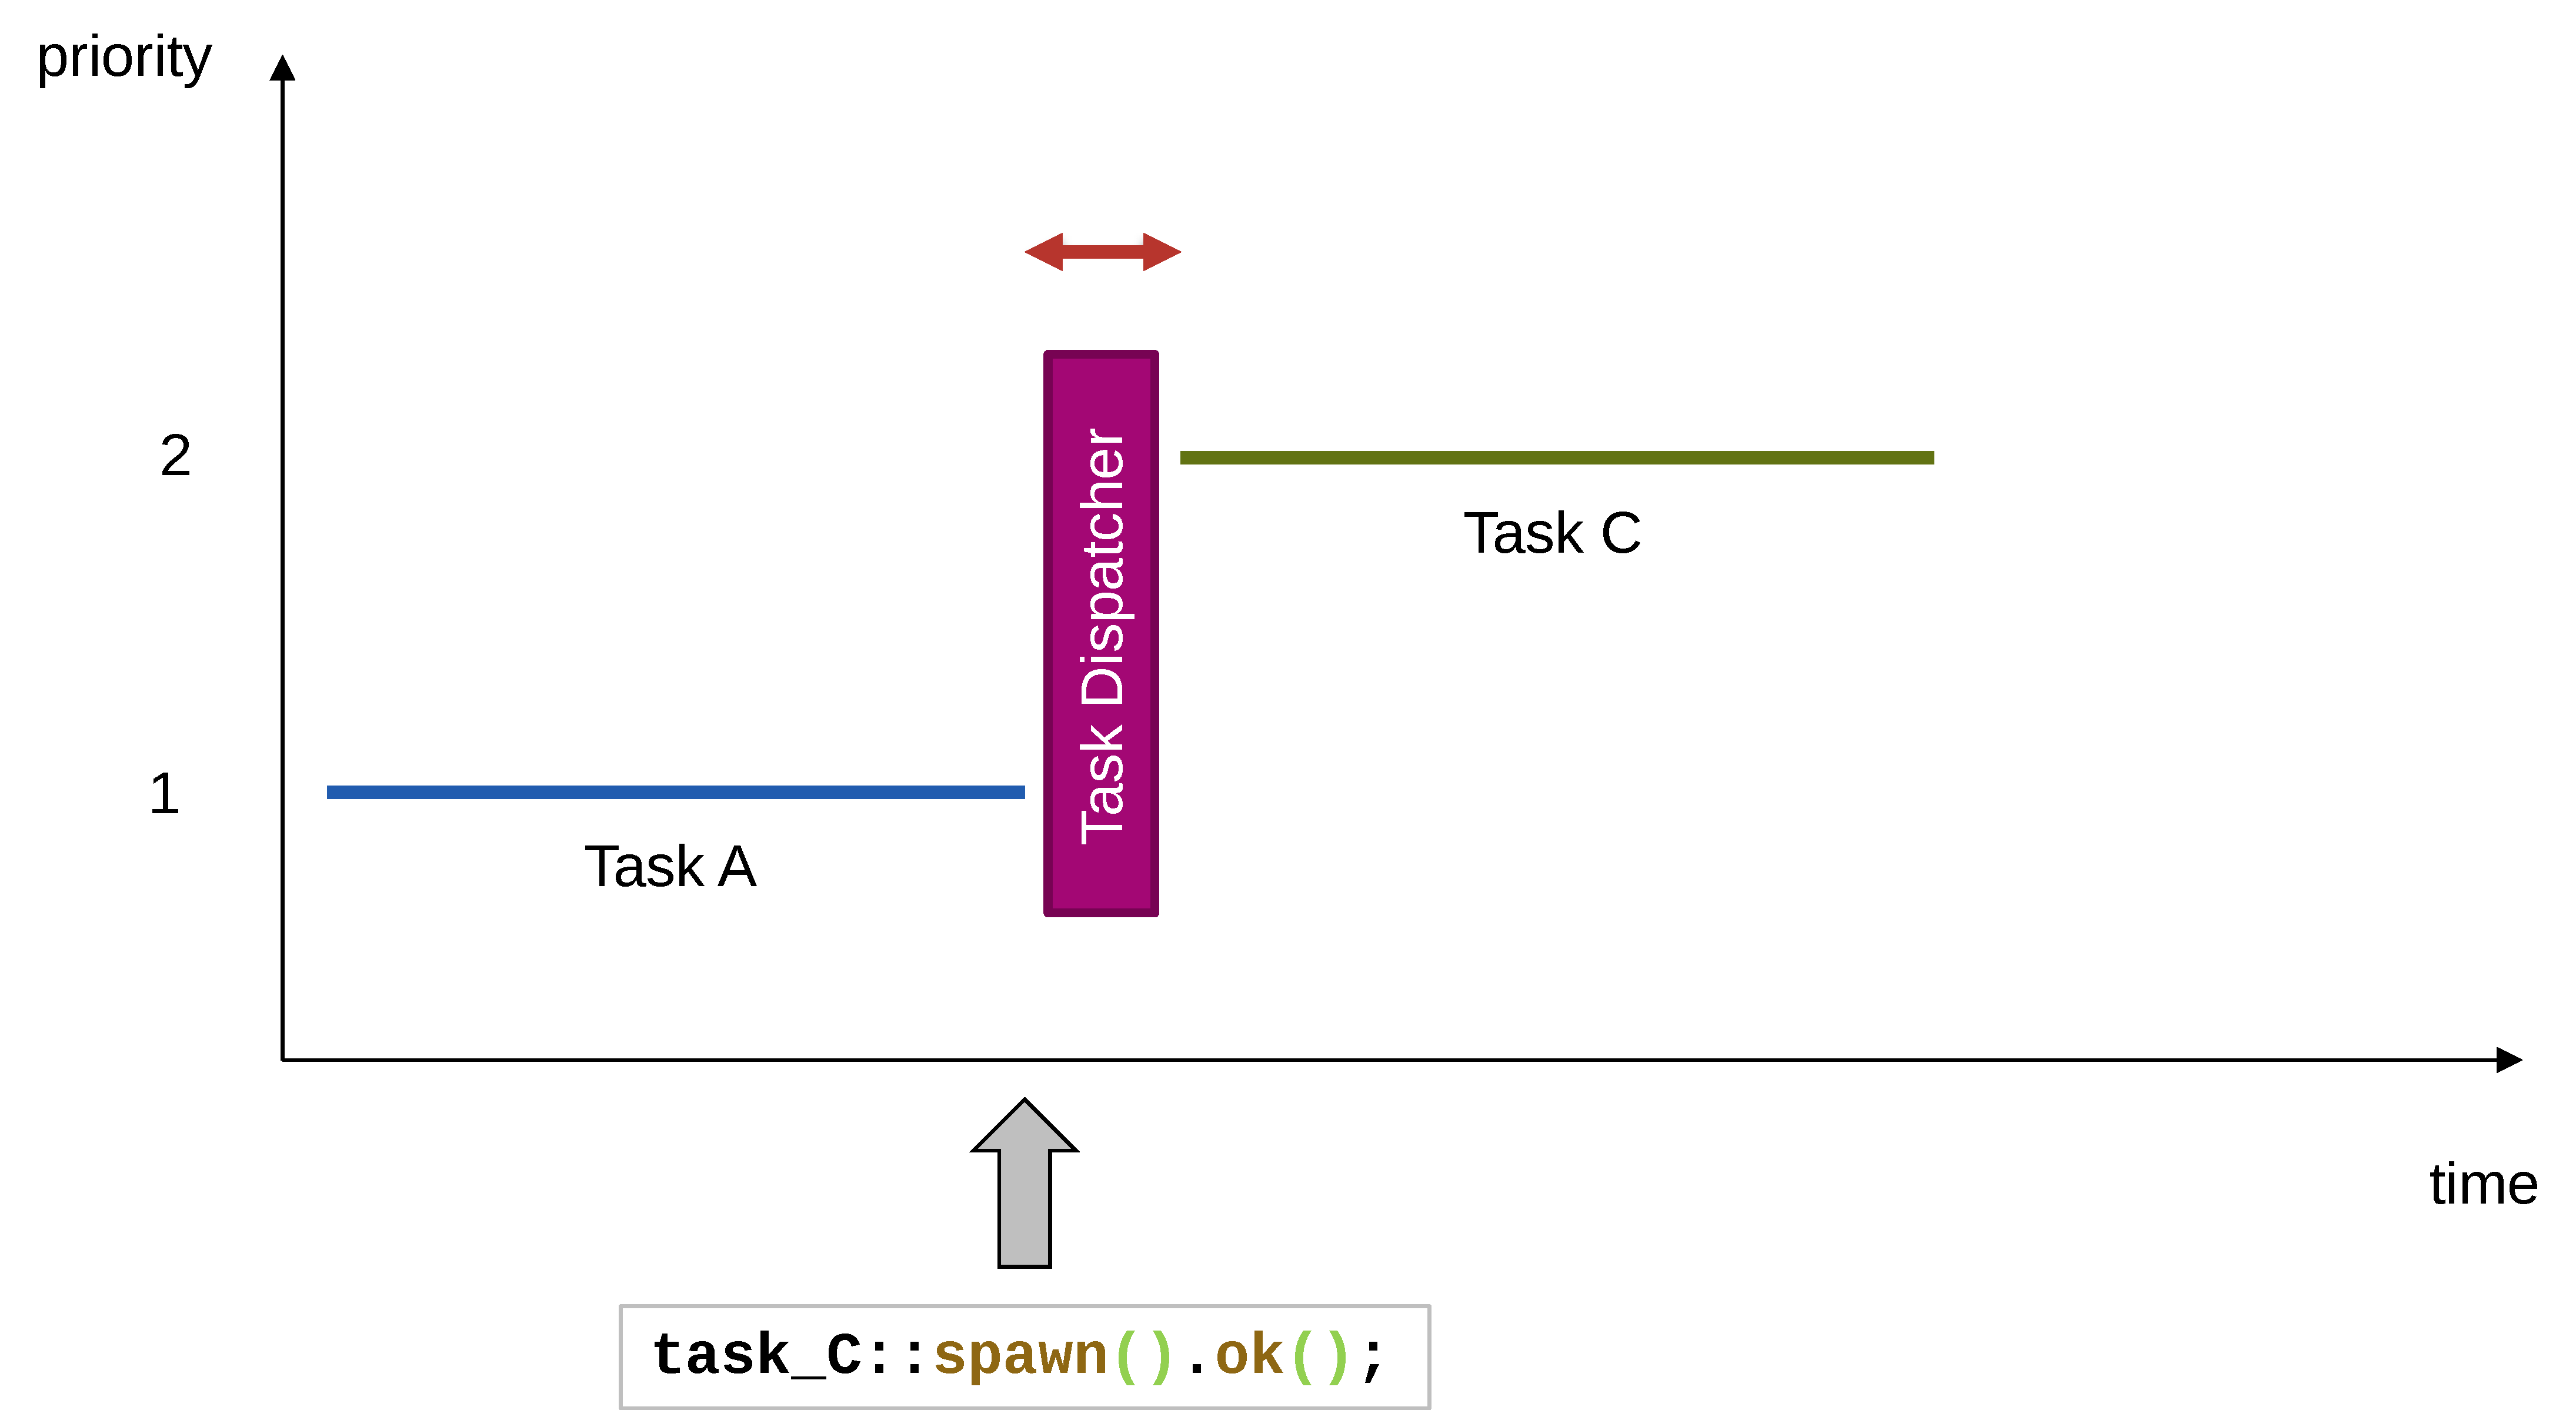
\includegraphics[width=\textwidth]{fig/spawn_prio_high.svg.pdf}
  % Note: We do not have the SVG source file for the image above, so we have to put the PDF under version control.
  \caption{Spawn Task with Higher Priority}%
  \label{fig:spawn_prio_high}
  % Note: The `\label{}` can be on the line after the `\caption{}` if the `\caption{}` line ends with a comment.
\end{figure}

If a task of higher priority (task C) is spawned, the original task is preempted immediately. See figure~\ref{fig:spawn_prio_high}.
We measured the cycles from directly before the execution of the \texttt{task_C::spawn().ok()} statement until the first instruction of the task C Rust function.
This includes the enqueuing of the task into the ready queue of the task dispatcher, the pending of the interrupt associated with the task dispatcher for priority 2, the context switch to the new interrupt handler, the dequeuing of task C, and finally, the prologue of the Rust function of task C.

\subsection{Task Spawn Lower Priority}

\begin{figure}
  \centerfloat
  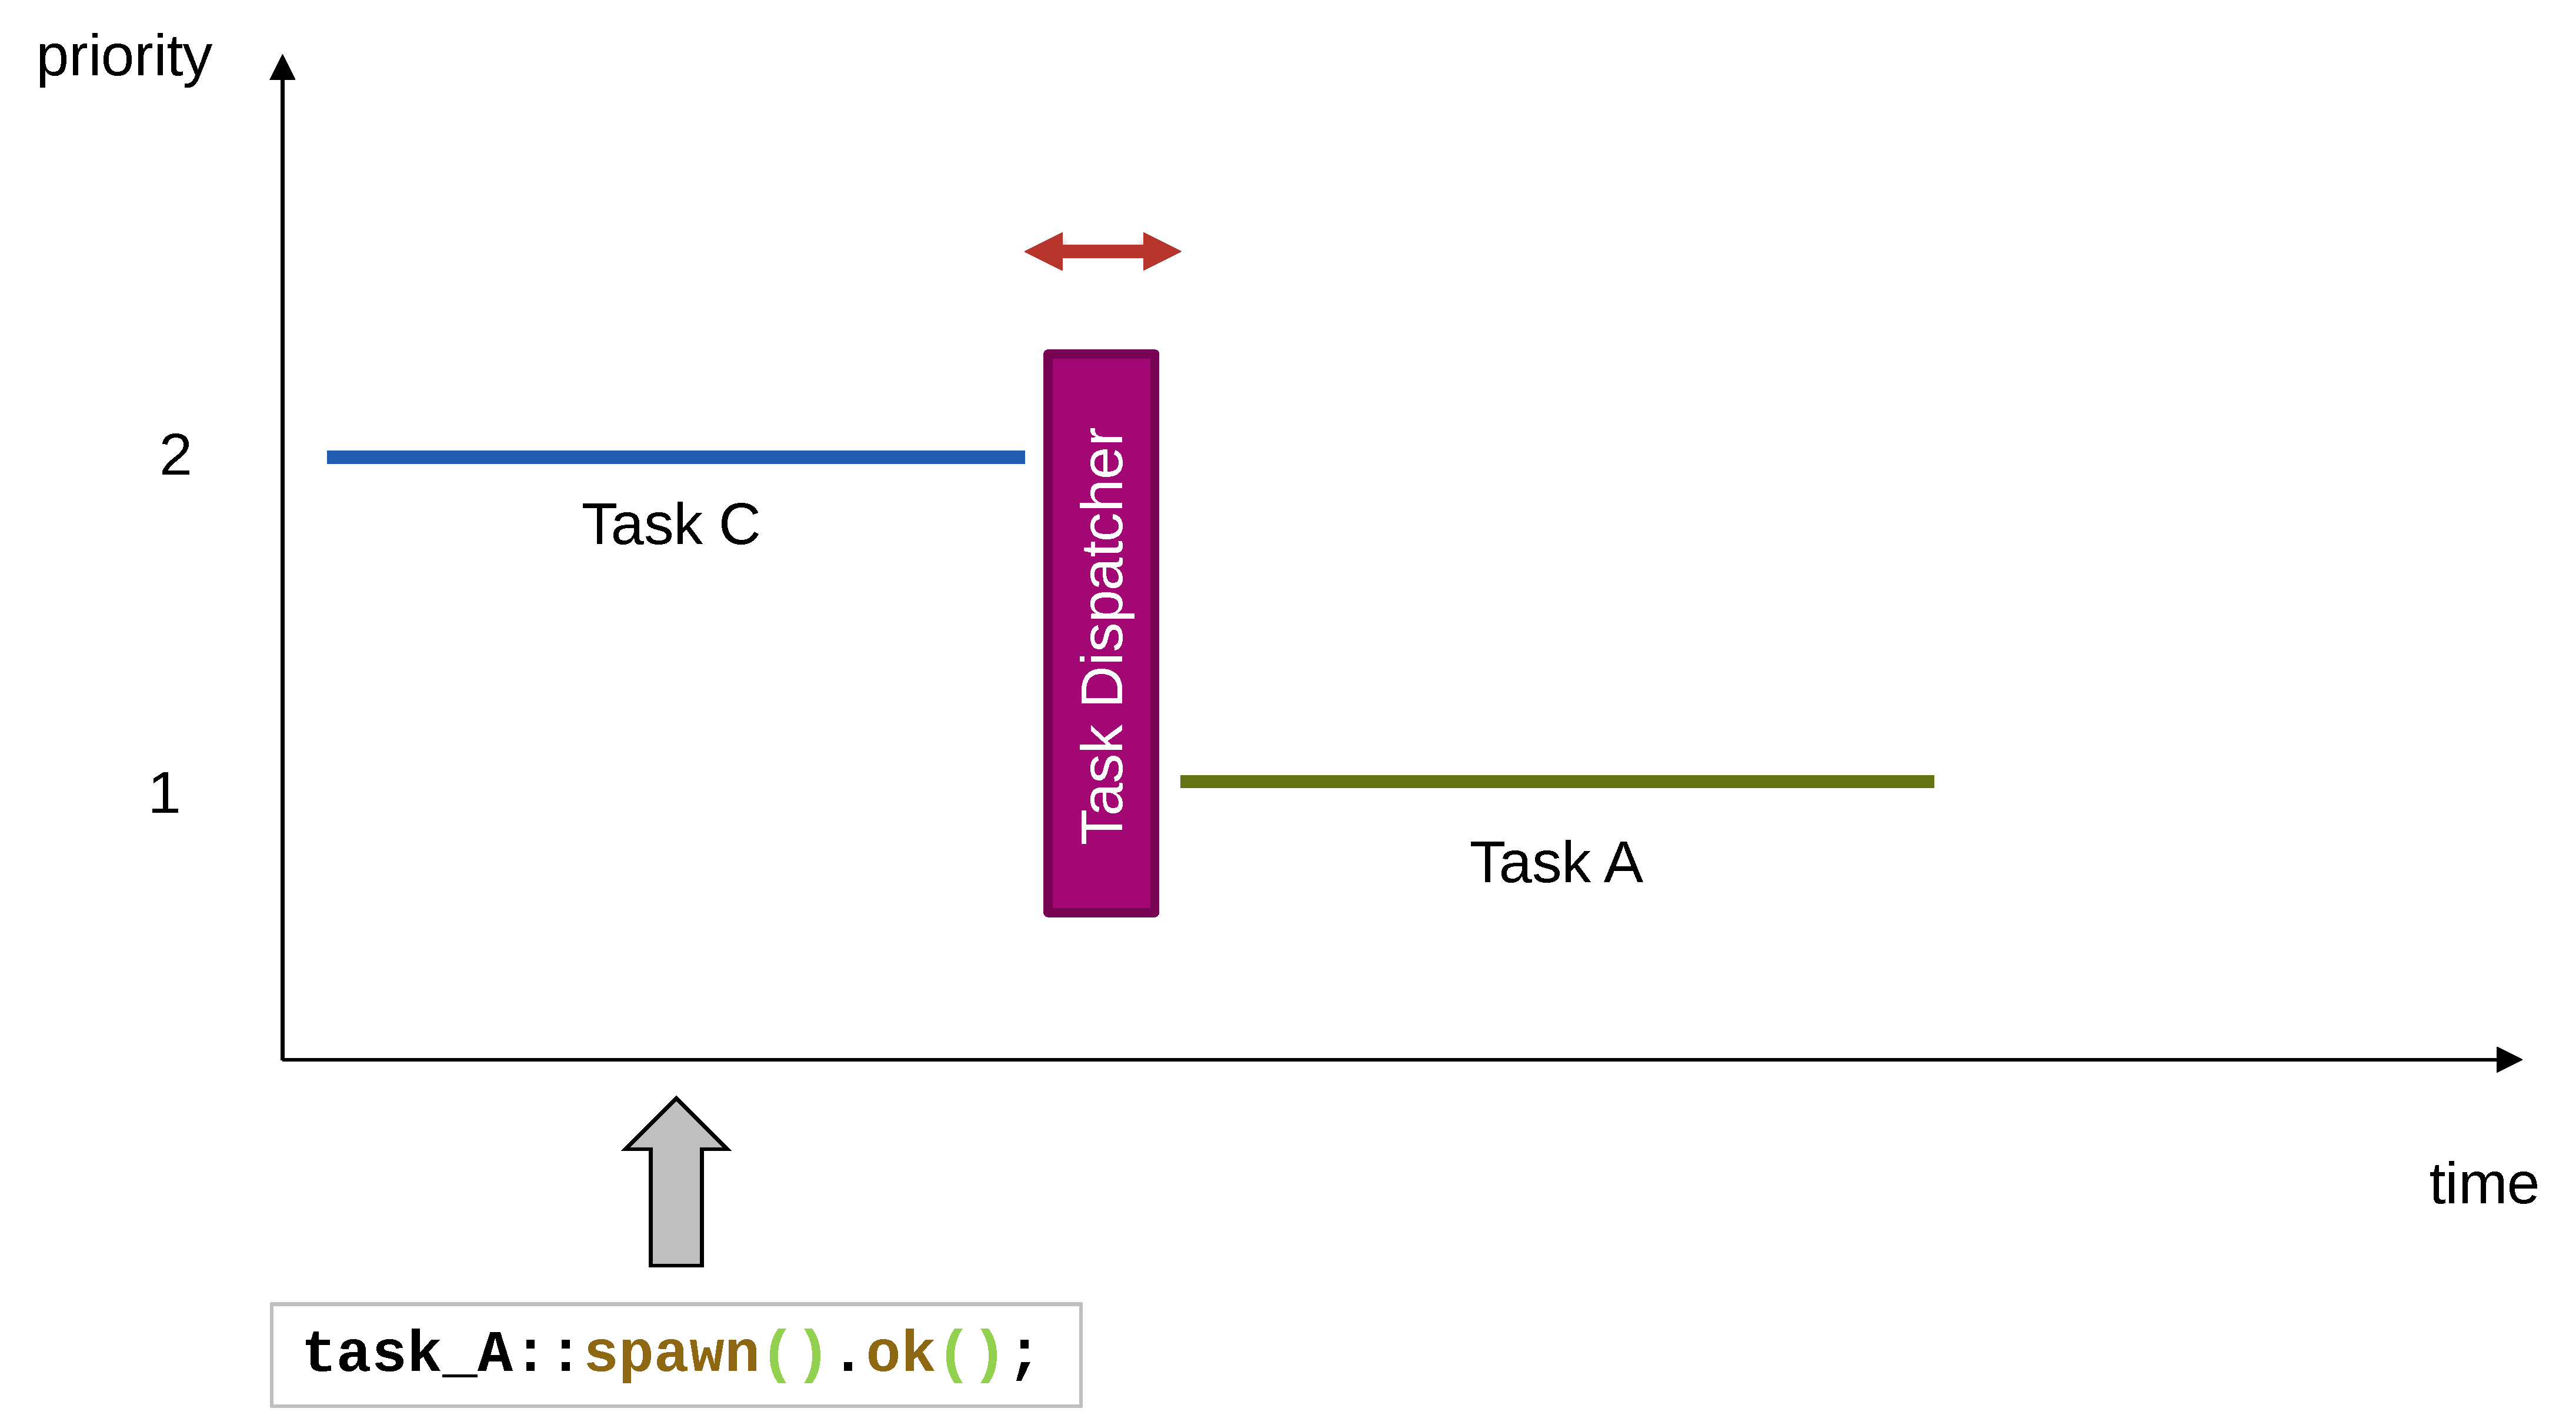
\includegraphics[width=\textwidth]{fig/spawn_prio_low.svg.pdf}
  % Note: We do not have the SVG source file for the image above, so we have to put the PDF under version control.
  \caption{Spawn Task with Lower Priority}%
  \label{fig:spawn_prio_low}
  % Note: The `\label{}` can be on the line after the `\caption{}` if the `\caption{}` line ends with a comment.
\end{figure}

If a task of lower priority is spawned (task A), the new task is enqueued into the ready queue of its task dispatcher, and the corresponding interrupt is pended in software. But since it has lower priority, it does not fire immediately, and the original task (task C) will finish execution first.
In this transition, we measure the cycles between the last instruction of the Rust function of task C and the first instruction of the Rust function of task A. See figure~\ref{fig:spawn_prio_low}.
This includes the epilogue of task C, the interrupt context switch, the dequeuing of task A and the prologue of task A.

\subsection{Task Spawn Equal Priority}

\begin{figure}
  \centerfloat
  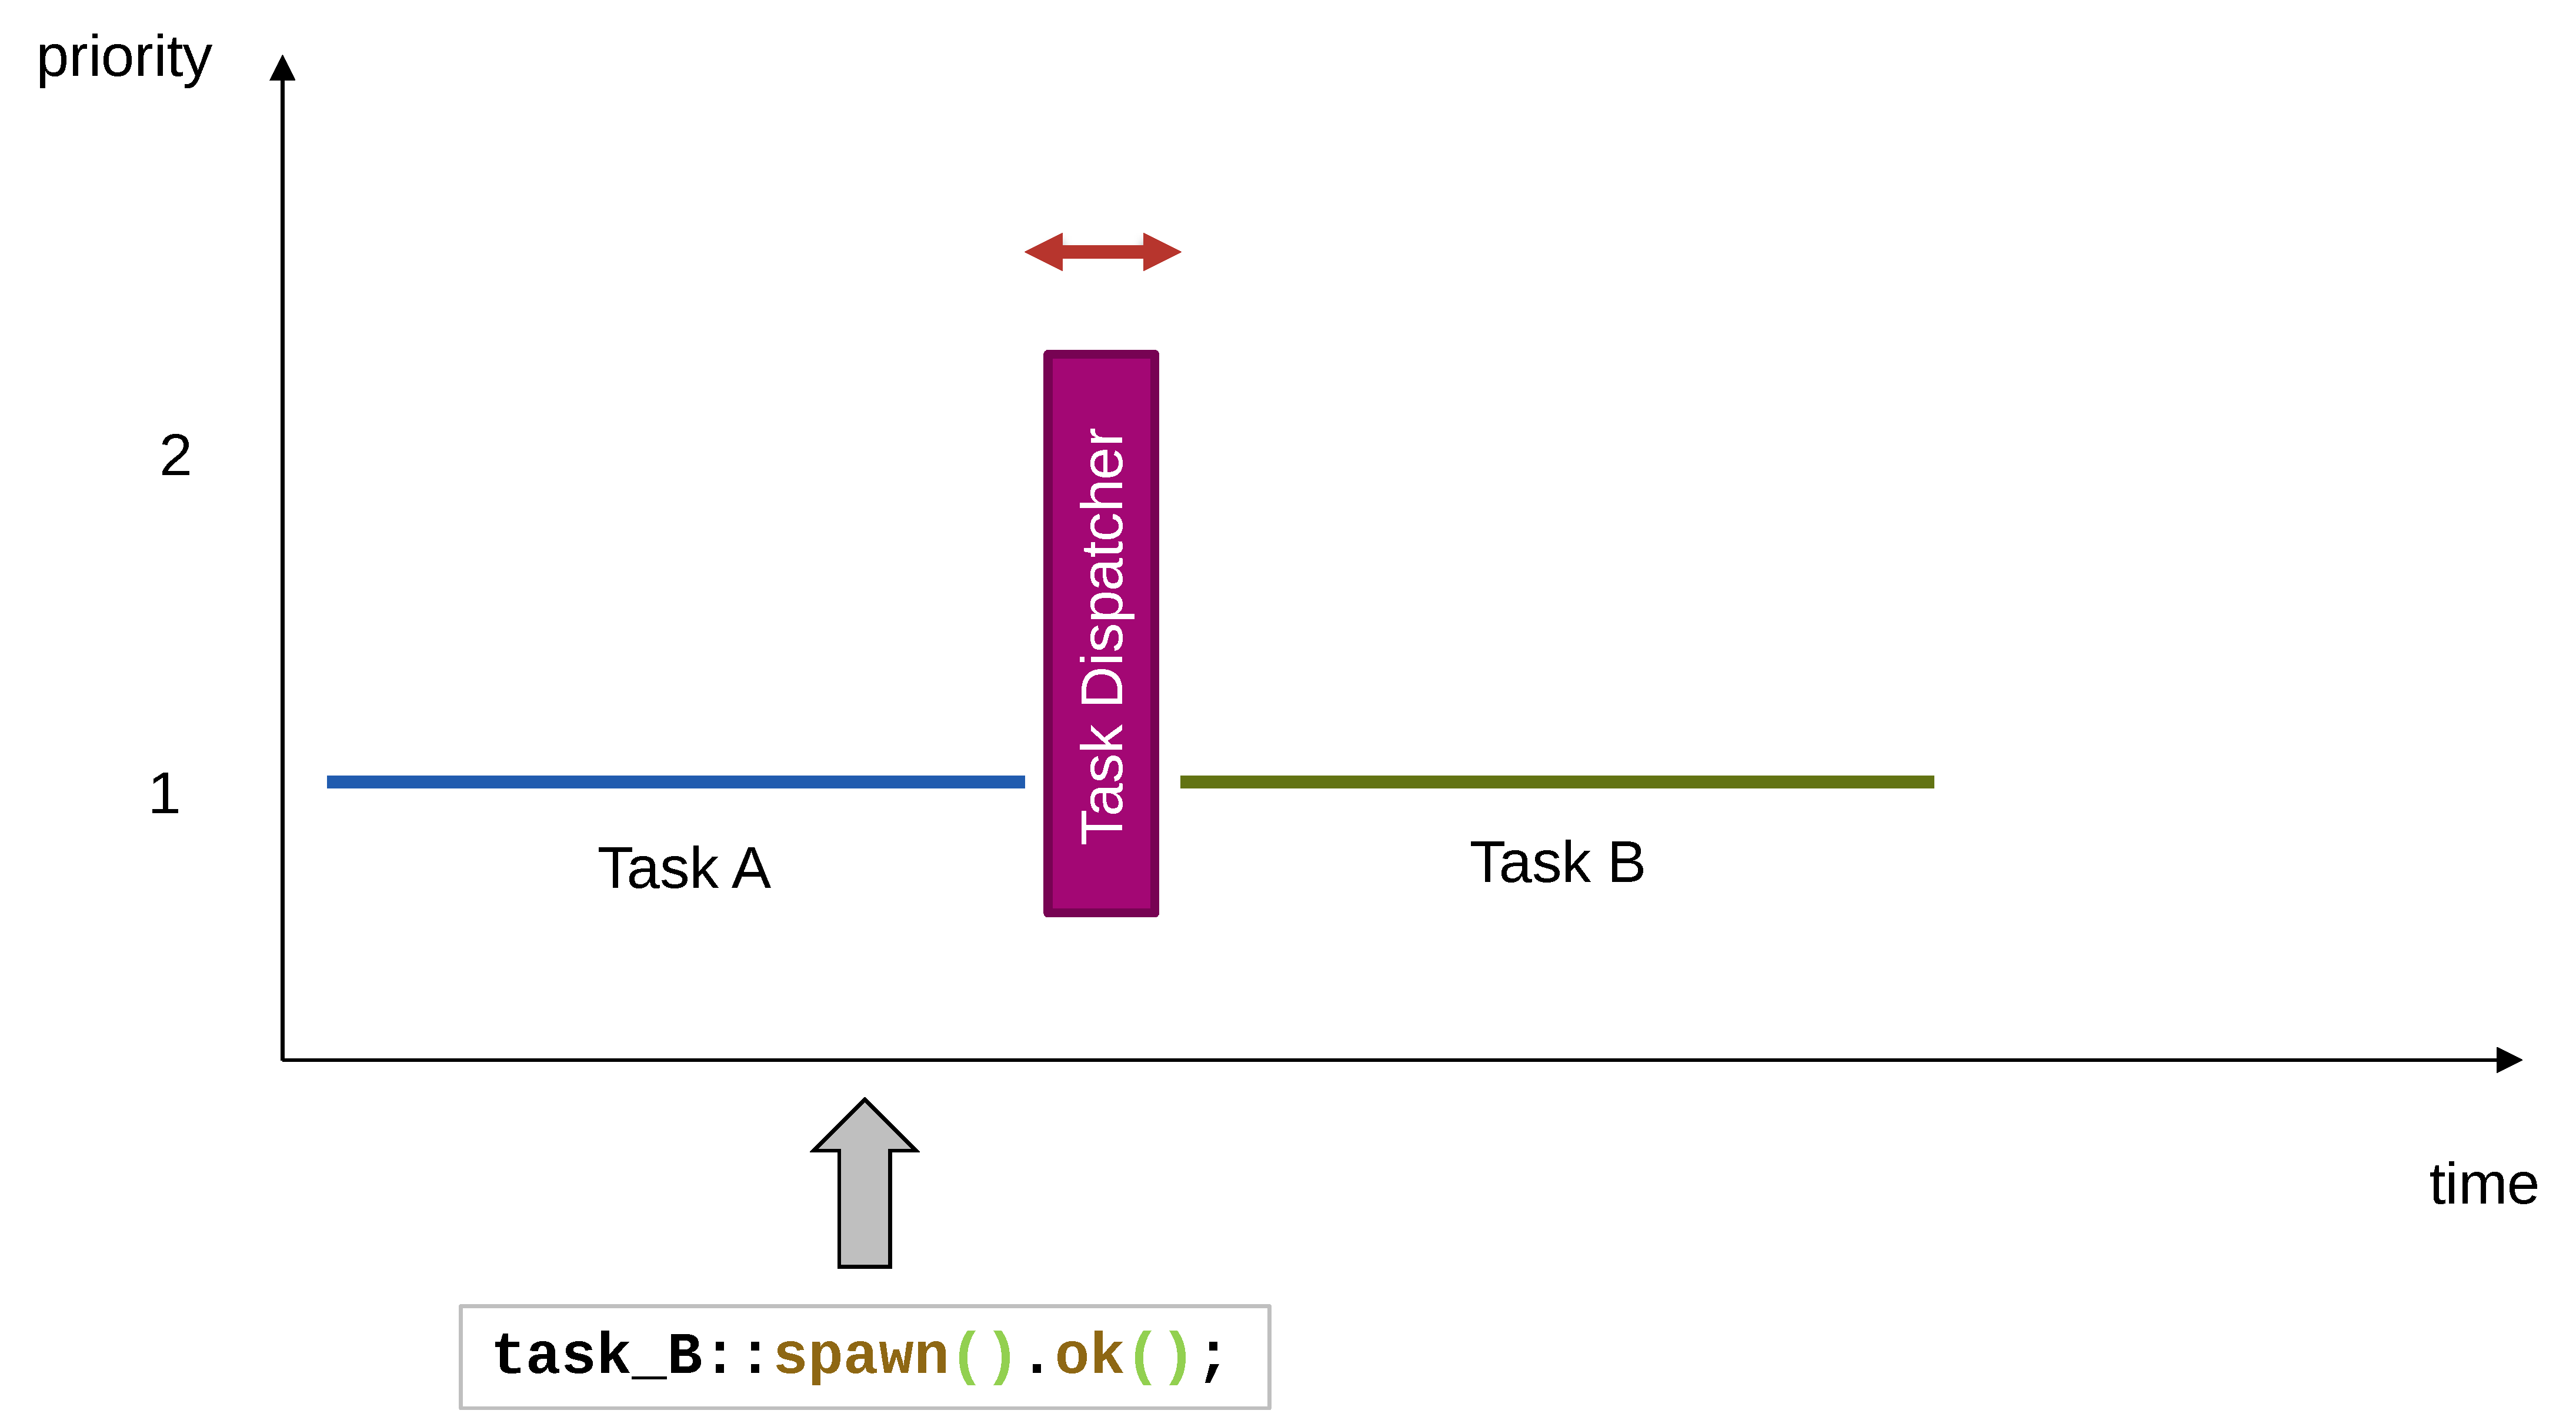
\includegraphics[width=\textwidth]{fig/spawn_prio_equal.svg.pdf}
  % Note: We do not have the SVG source file for the image above, so we have to put the PDF under version control.
  \caption{Spawn Task with Equal Priority}%
  \label{fig:spawn_prio_equal}
  % Note: The `\label{}` can be on the line after the `\caption{}` if the `\caption{}` line ends with a comment.
\end{figure}

If a task of equal priority (task B) is spawned, the new task is enqueued into the ready queue of its task dispatcher, and the corresponding interrupt is pended in software. However, since there is only one task dispatcher per priority, the pended interrupt is actually the same that is currently being handled. This means, that the current task (task A) will run until completion. Then the task dispatcher that is already running will dequeue the new task and run it directly. So no context switch is necessary. Therefore, we measure the number of cycles between the last instruction of task A and the first instruction of task B. See figure~\ref{fig:spawn_prio_equal}.

This includes the epilogue of task A, the dequeuing of task B and the prologue of task B.

\subsection{Timed Task Spawn}

\begin{figure}
  \centerfloat
  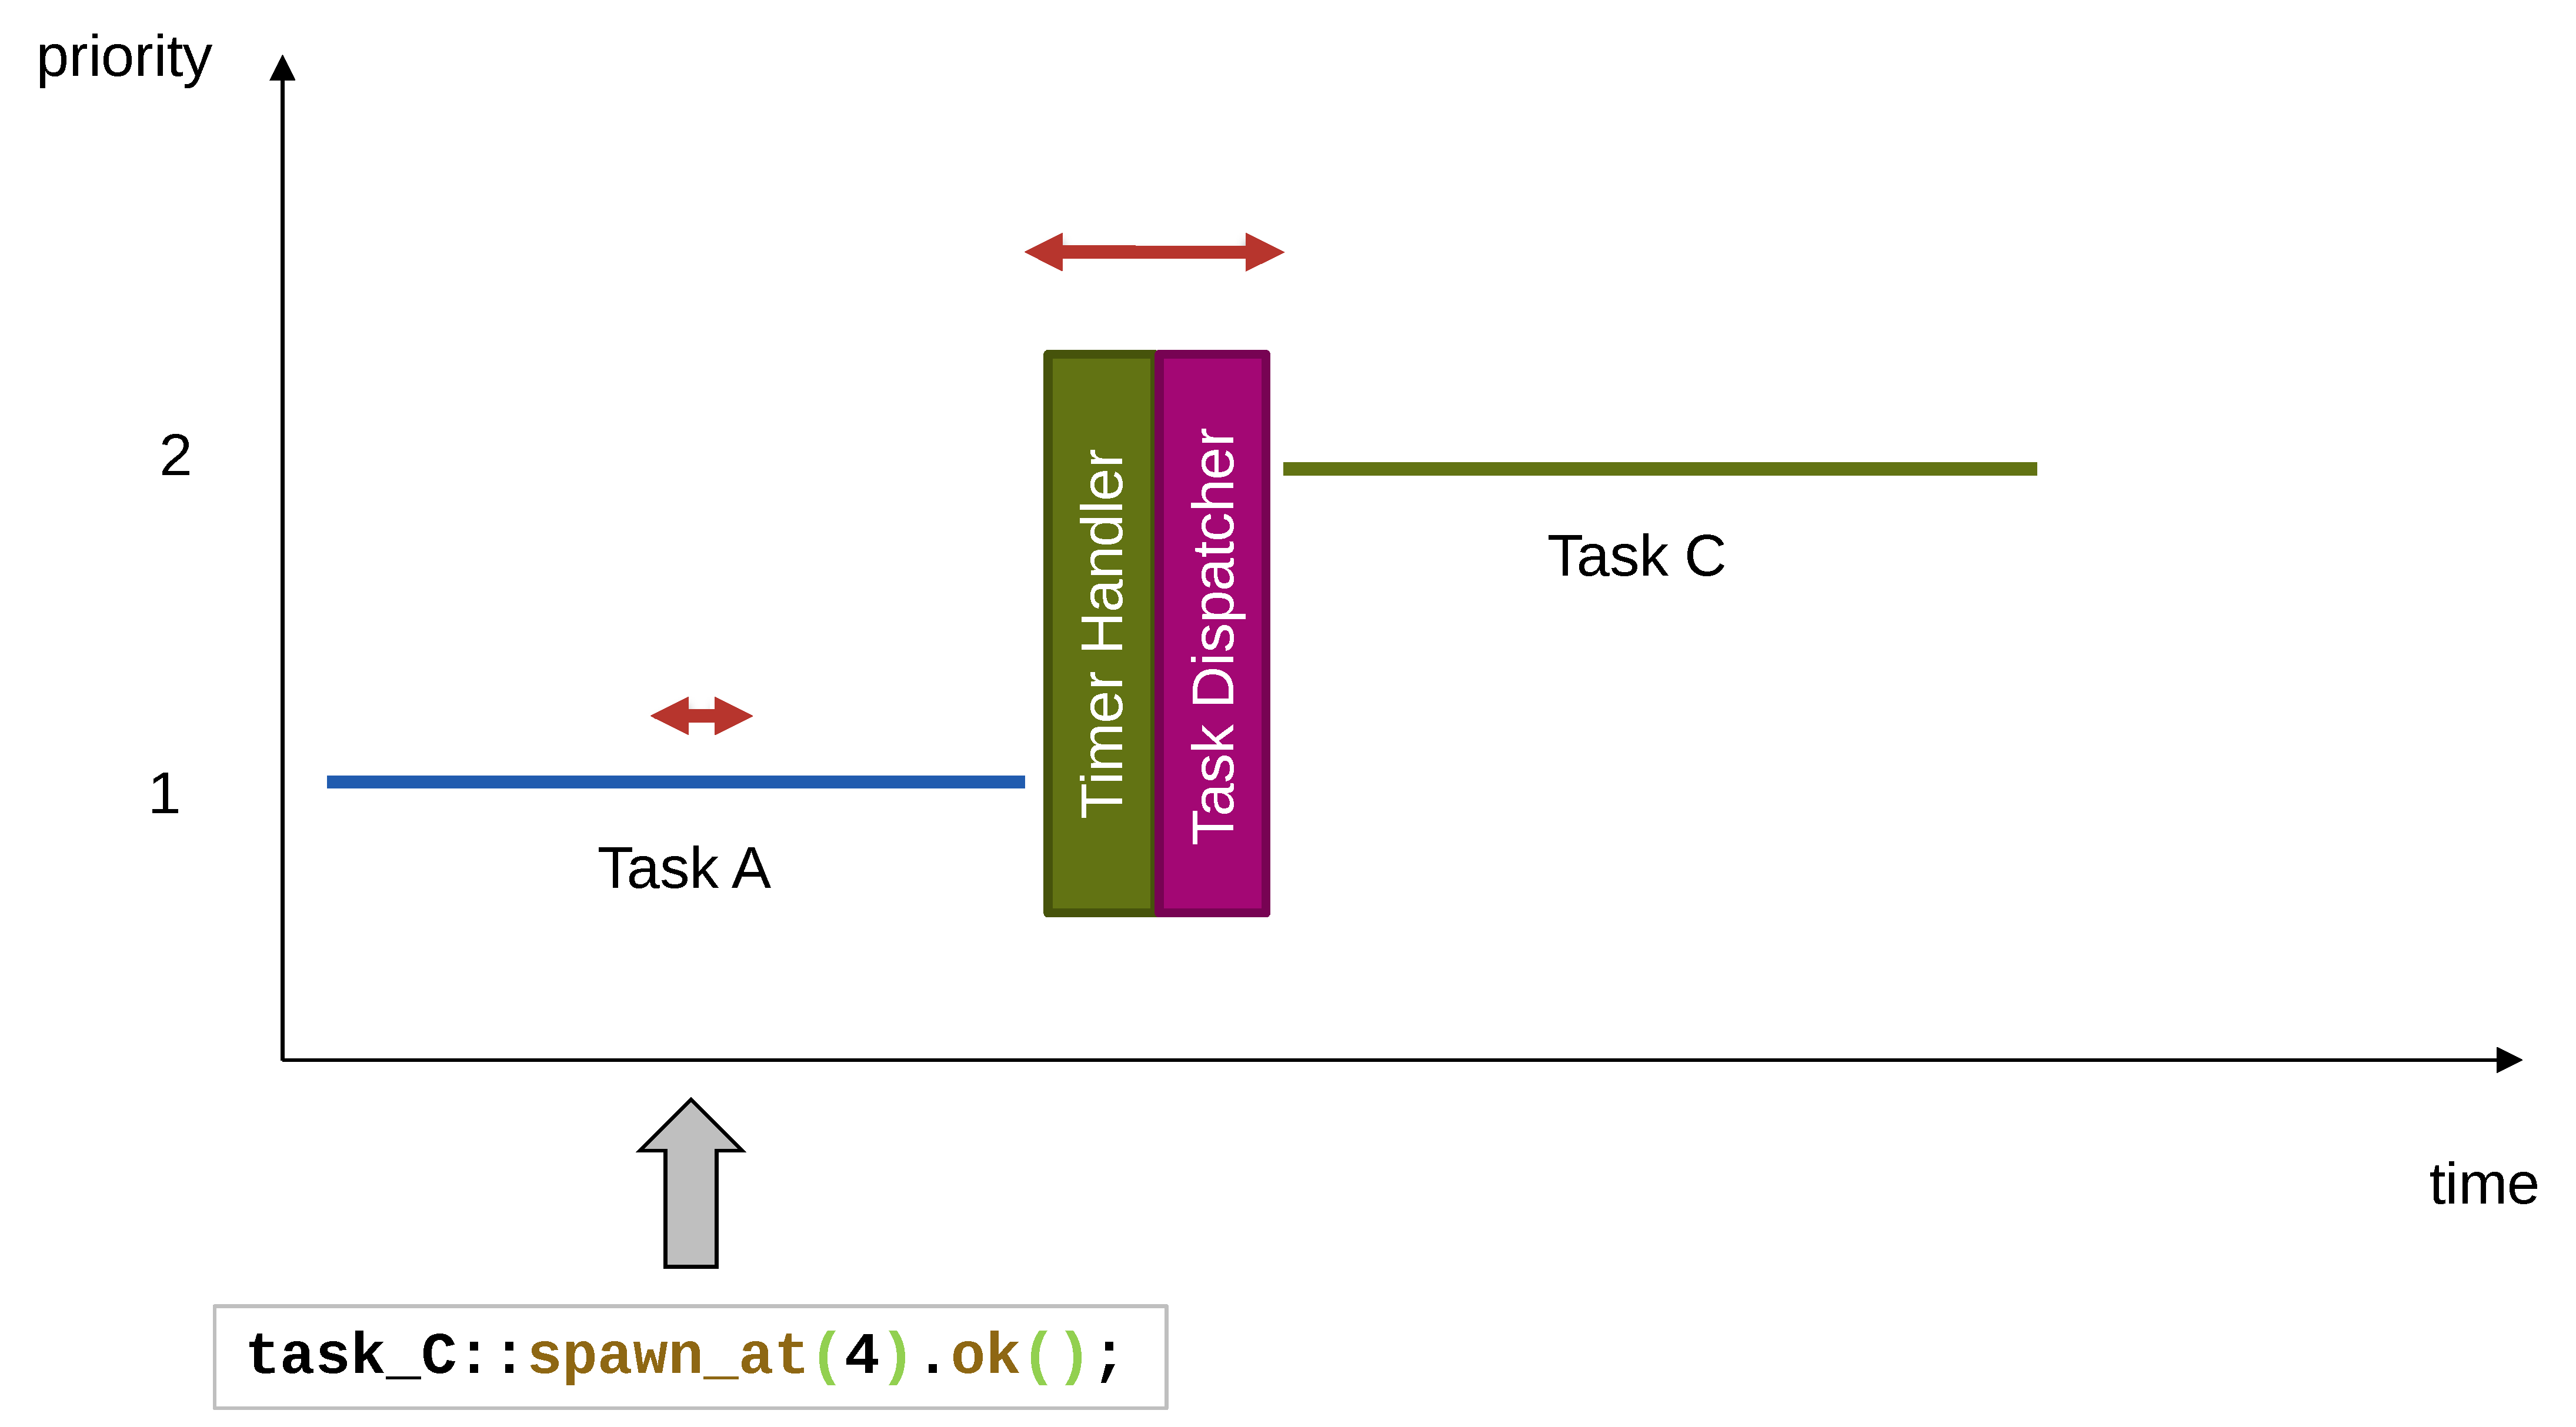
\includegraphics[width=\textwidth]{fig/spawn_prio_timed.svg.pdf}
  % Note: We do not have the SVG source file for the image above, so we have to put the PDF under version control.
  \caption{Spawning of a Timed Task}%
  \label{fig:spawn_prio_timed}
  % Note: The `\label{}` can be on the line after the `\caption{}` if the `\caption{}` line ends with a comment.
\end{figure}

In the spawning process of a timed task (task C), there are two interesting sequences to measure. First, the scheduling of task C. And secondly, the effective start time of task C. See figure~\ref{fig:spawn_prio_timed}.

For the scheduling, the task first is sorted into the timer queue. Then, the timer comparison value is set to the spawn point of the first task in the sorted timer queue. It could actually be finished now, but to catch edge cases, a few safety operations are performed.

Therefore, the timer interrupt is pended, and the context is switched to the timer interrupt. It checks if its first task is already due (which it normally is not, it is only done to catch tasks that are scheduled in the past or very near future), and switches the context back to the original task (task A).

So the cycles between the last instruction before the \texttt{task_C::spawn_at(4).ok} statement and the first instruction after it are measured. This spawning procedure can seam quite inefficient, but it is given by \gls{rtic}.

For the actual starting of task C, we measure the cycles from the point where the timer fires to the first instruction of the Rust function of task C.
This includes the context switch to the timer handler, the dequeuing of task C from the timer queue, the enqueuing of task C into the ready queue of its task dispatcher, the pending of the task dispatcher, the context switch into the task dispatcher's interrupt handler, the dequeuing of task C from the ready queue and finally the prologue of task C.

\subsection{Locking}

Besides the spawning of tasks, sharing resources among tasks is one of the most important processes in operating systems. Therefore, we measure the locking and unlocking overhead of a resource. Since in \gls{rtic} it makes a difference if the locking happens in the task with the highest priority that has access to a specific resource, or in any other task, we measure both cases, see figures~\ref{fig:locking_high_prio} and \ref{fig:locking_low_prio}.

Here, we measure the number of cycles between the last instruction before the locking/unlocking statement and the first instruction after the locking/unlocking statement.

To get a better understanding of how locking of shared resources works in \gls{rtic}, refer to section \ref{sec:shared_resources}.

\begin{figure}
  \centerfloat
  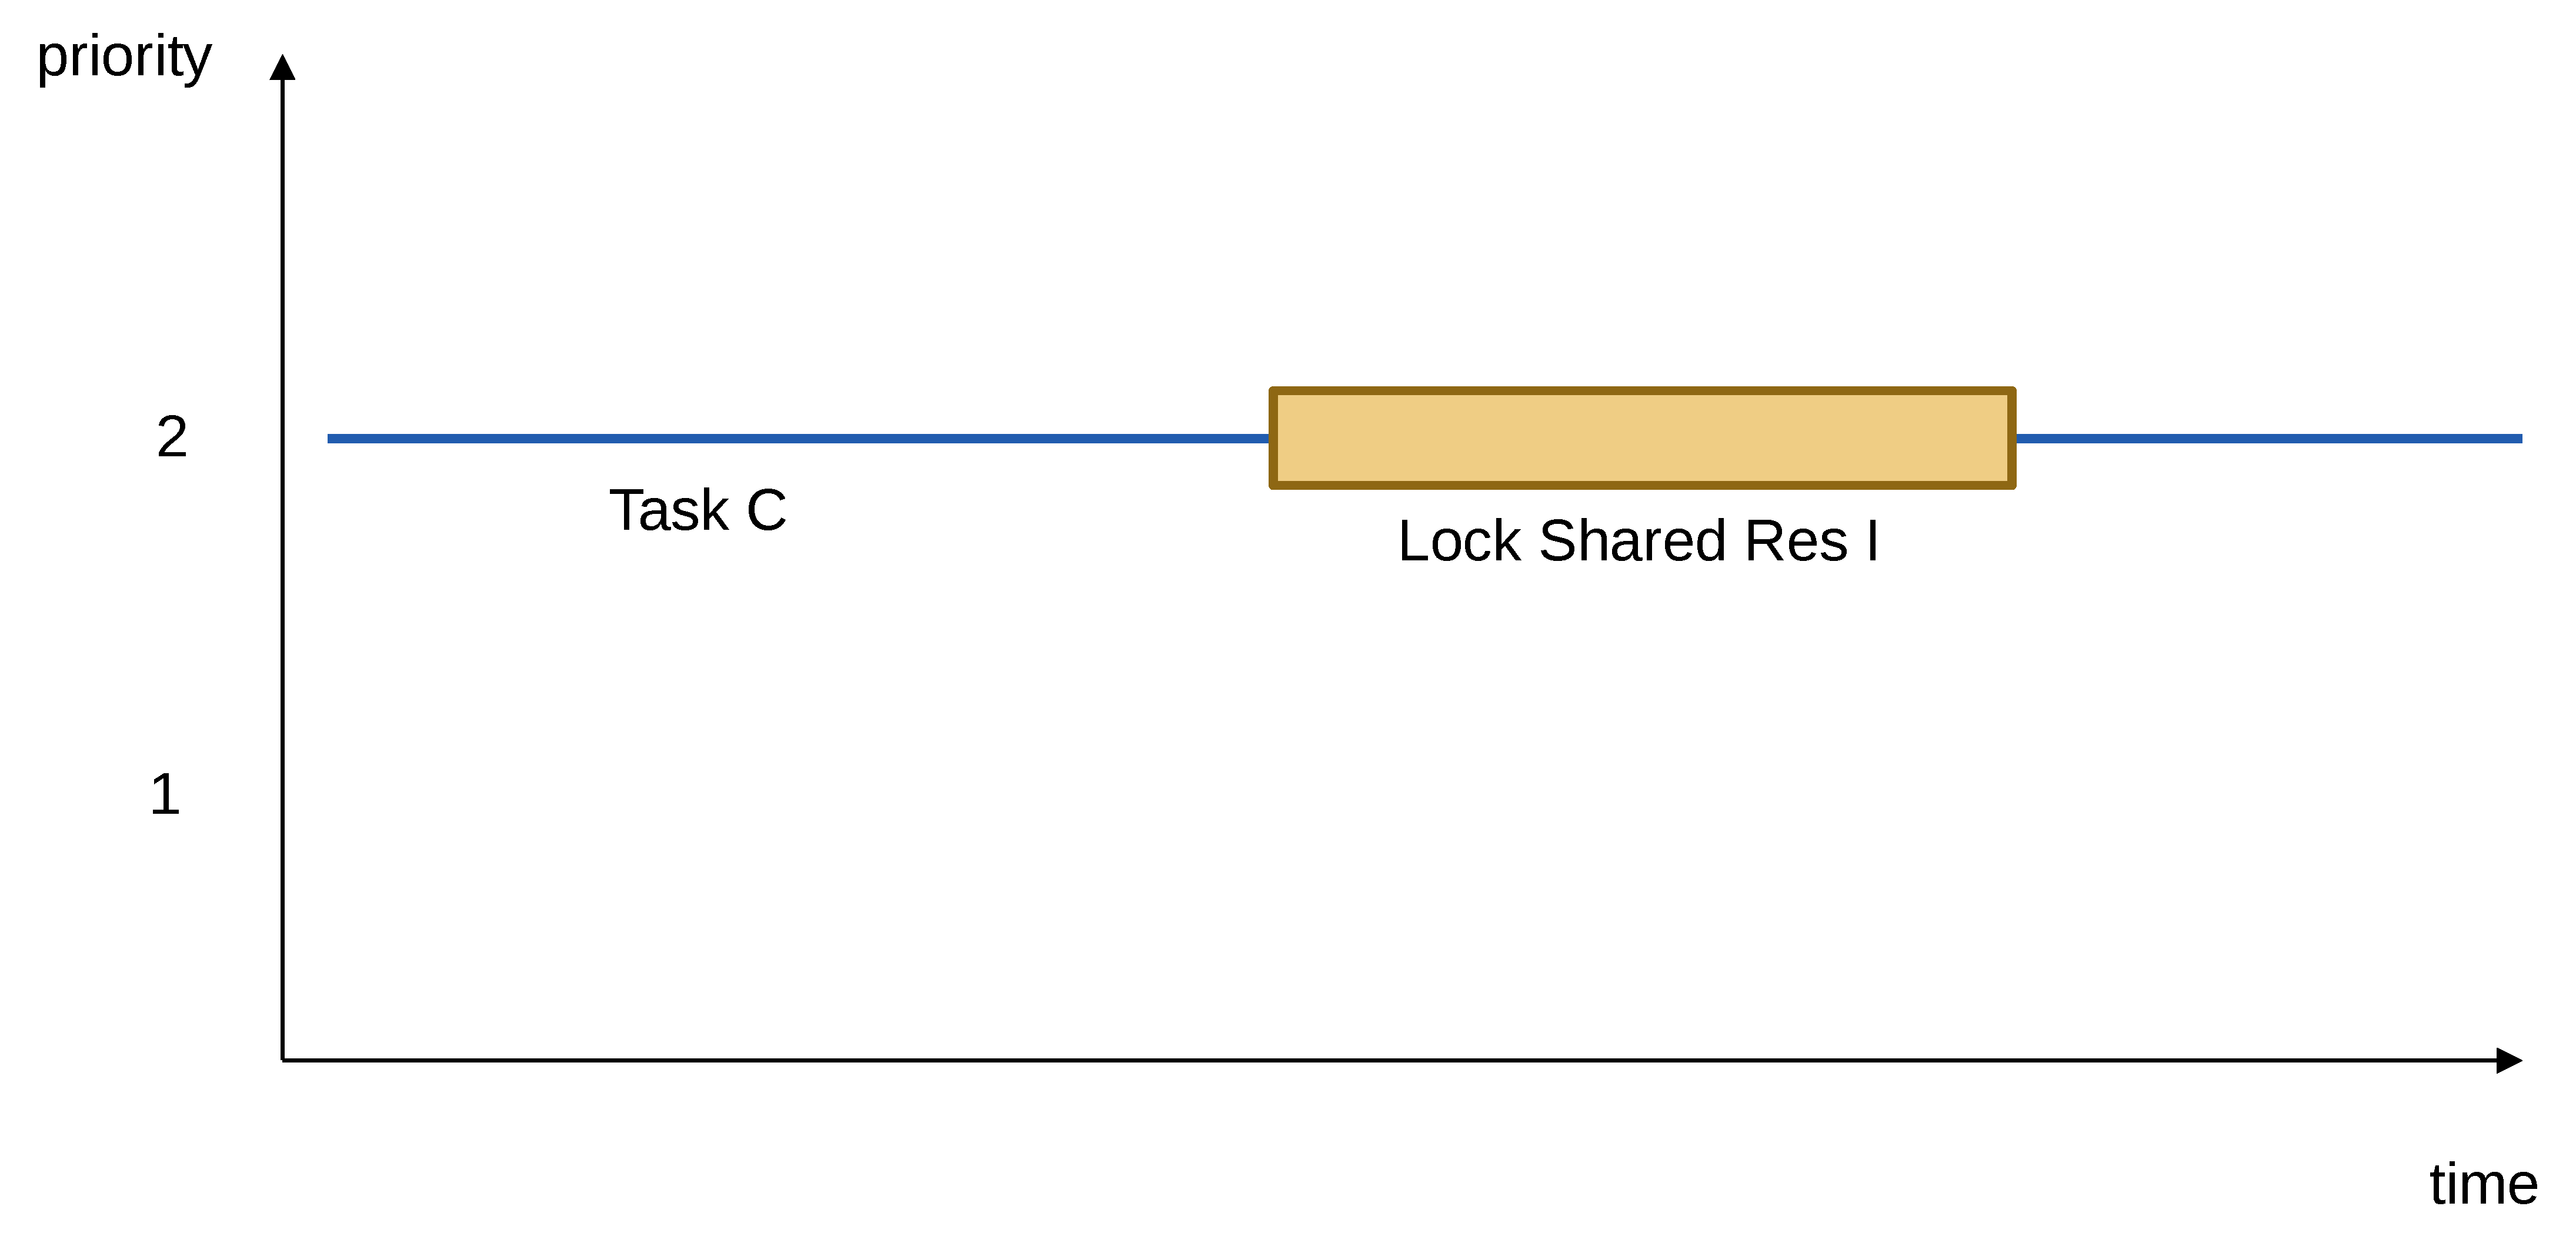
\includegraphics[width=\textwidth]{fig/locking_high_prio.svg.pdf}
  % Note: We do not have the SVG source file for the image above, so we have to put the PDF under version control.
  \caption{Locking of a Resource as highest Priority Task}%
  \label{fig:locking_high_prio}
  % Note: The `\label{}` can be on the line after the `\caption{}` if the `\caption{}` line ends with a comment.
\end{figure}

\begin{figure}
  \centerfloat
  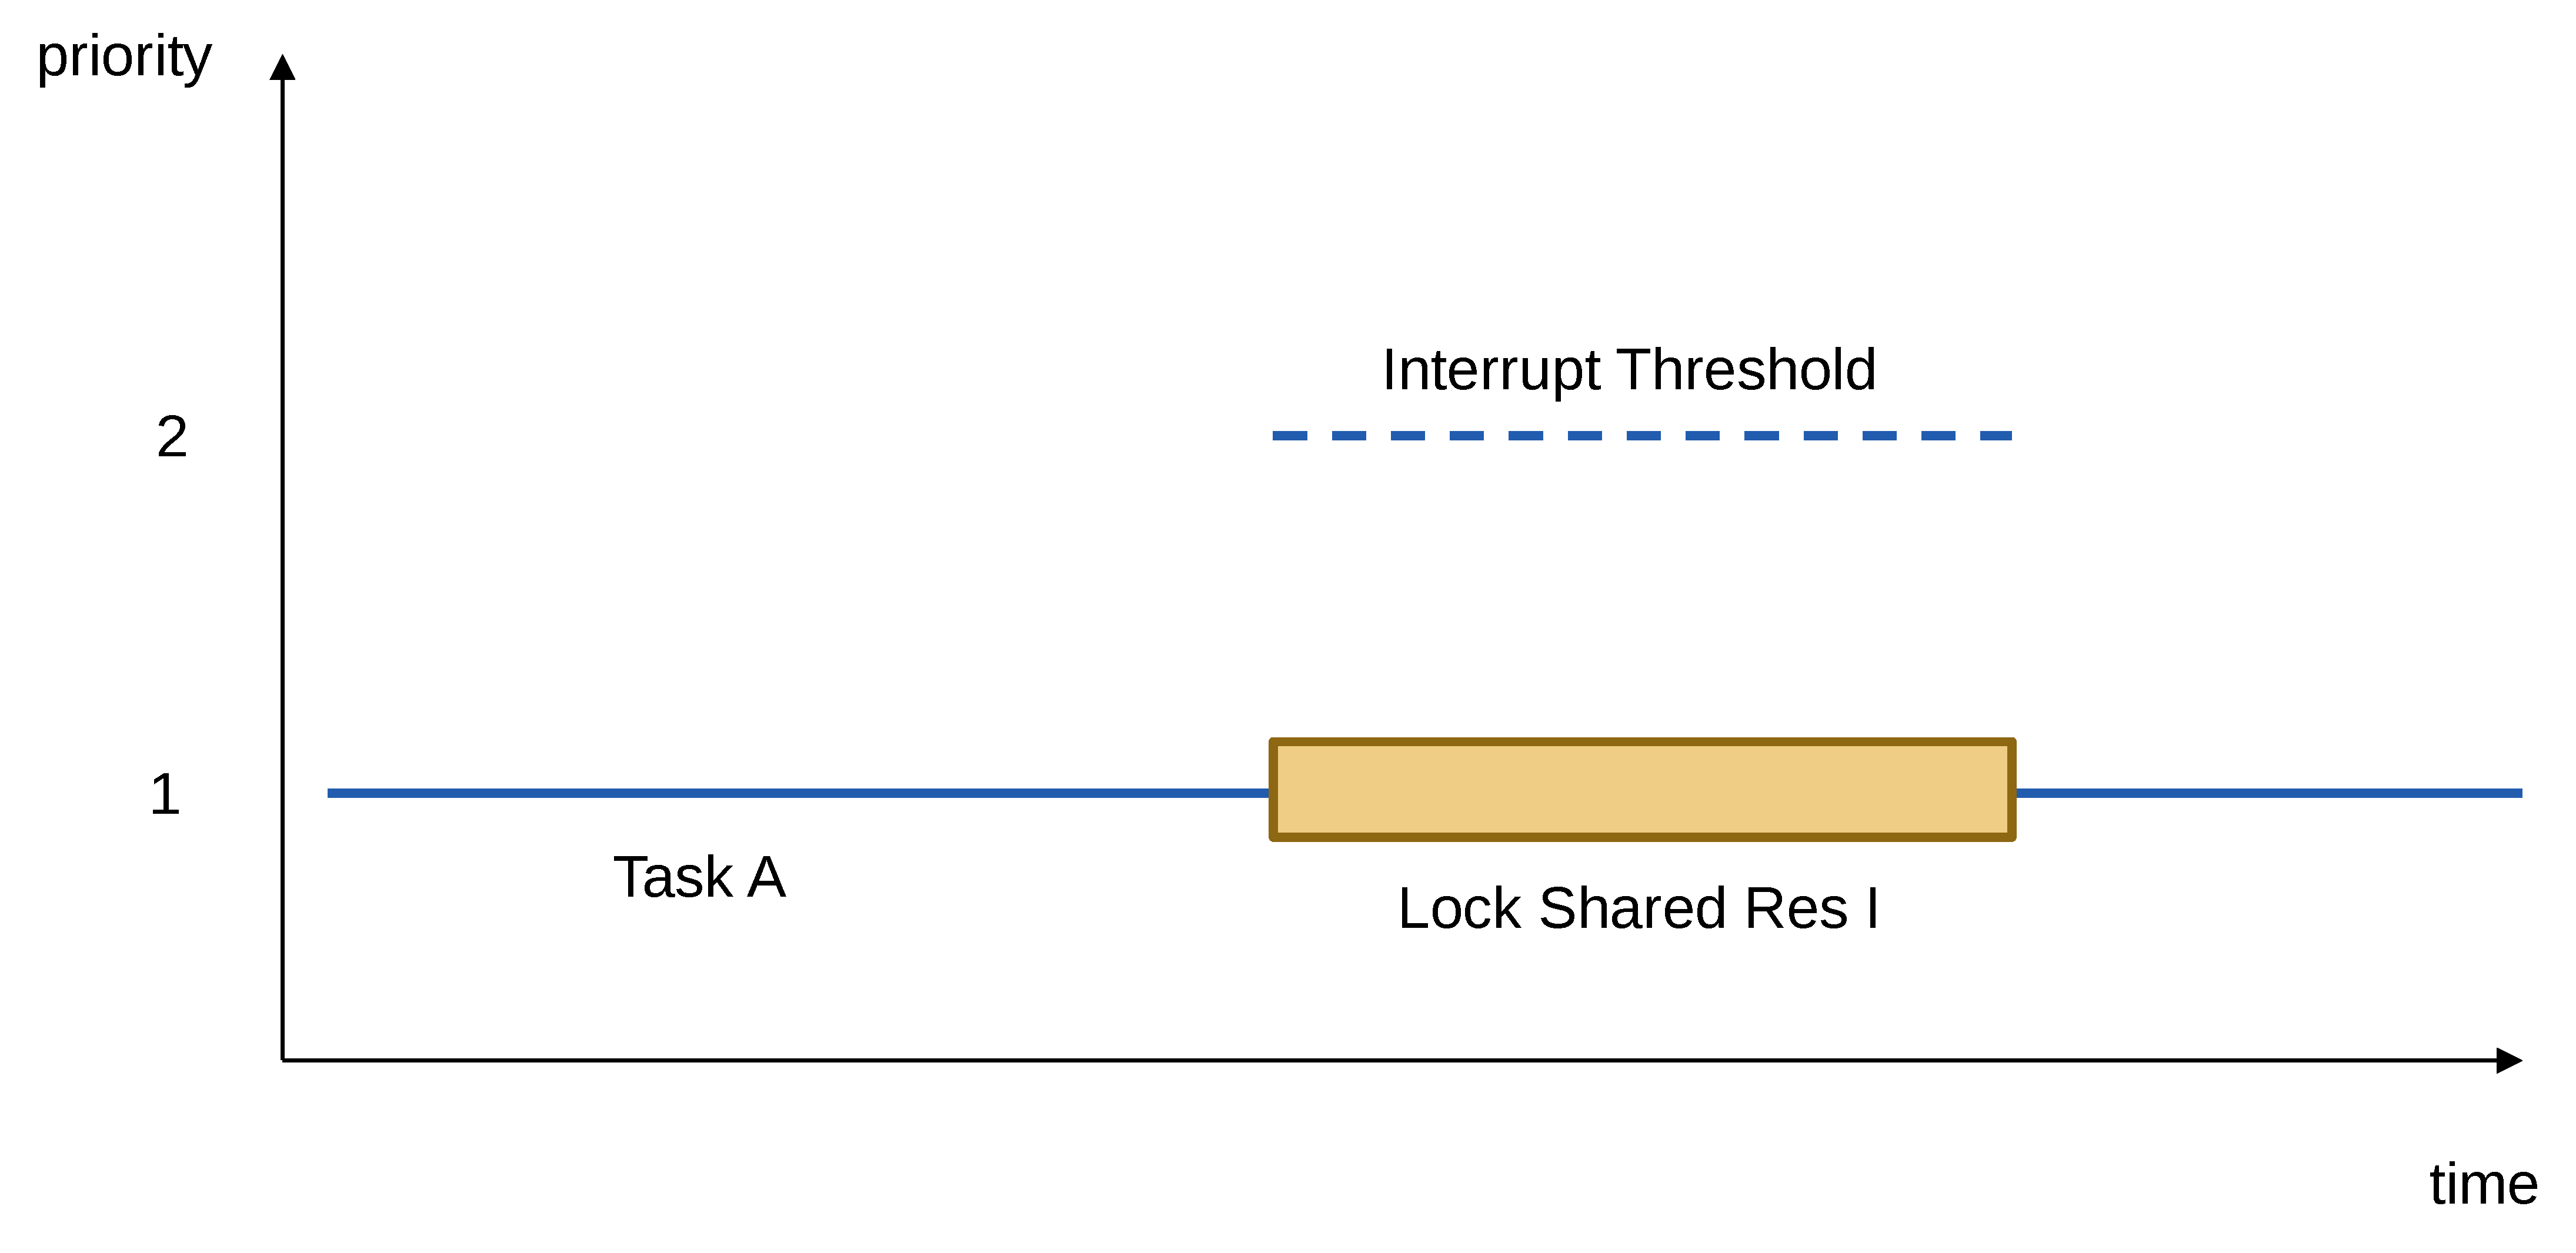
\includegraphics[width=\textwidth]{fig/locking_low_prio.svg.pdf}
  % Note: We do not have the SVG source file for the image above, so we have to put the PDF under version control.
  \caption{Locking of a Resource}%
  \label{fig:locking_low_prio}
  % Note: The `\label{}` can be on the line after the `\caption{}` if the `\caption{}` line ends with a comment.
\end{figure}

\section{Measurement Results}

In the following section, the results of the measurements that are described in section~\ref{sec:core_transitions} are presented.

Since locking of shared resources is already highly optimized by \gls{rtic}, it only uses between about zero and four cycles, which is in the same range as the measurement uncertainties, see section~\ref{sec:time_measurement}. Therefore, we do not show the locking measurements in the plots below, since they do not include any meaningful information.

\subsection{Original Implementation}
\label{sec:results_original_implementation}

In the plot in figure~\ref{fig:plot_original}, one can see the number of cycles that are used by the operations described in section~\ref{sec:core_transitions}. It is clearly visible that the implementation for ARM outperforms the one for RISC-V if the original implementation with the integer ABI is used. The exact cycle count number can be found in table~\ref{tbl:detailed_results}.

We identify two main differences. First, \gls{rtic} needs a 32bit timer for its timer handler. RISC-V already provides this, and therefore no overhead is added. In ARM, however, there exists only a 24bit timer. Therefore, the 32bit functionality had to be added in software. This leads to an overhead and explains why the RISC-V implementation performs better in scheduling timed tasks.

The vastly better performance of the ARM implementation can be explained with the much more performant interrupt handling in ARM. First, it has to be noted, that in ARM, interrupt context switching is handled in hardware, where it is parallelized. In RISC-V however, it is done in software, as explained in section~\ref{sec:interrupt_handler_macro}.

However, we developed hardware and software optimizations for the \gls{clic}.
See sections \ref{sec:results_nxti} and \ref{sec:results_fastirq} for results with an optimized RISC-V setup.


\begin{figure}
\begin{tikzpicture}
\begin{axis}[
	x tick label style={
		/pgf/number format/1000 sep=},
	ylabel=Cycle Count,
	enlargelimits=0.05,
	legend style={at={(0.5,1.1)},
	anchor=north,legend columns=-1},
        ybar=0cm,
        xtick=data,
        %xmajorgrids=true,
        width=\textwidth,
        enlarge x limits={abs=0.8},
        xticklabels={Hardware Task, Higher Prio Task, Equal Prio Task , Lower Prio Task, Scheduling Timed Task, Start Timed Task},
        xticklabel style={rotate=45, anchor=east},
]
\addplot [draw=none,fill=ETHBlue]
	coordinates {(0,32) (1,143)
		 (2,43) (3,106) (4,322) (5,332)};
\addplot [draw=none,fill=ETHRed]
	coordinates {(0,58) (1,170)
		 (2,51) (3,178) (4,307) (5,372)};
\legend{Arm Cortex-M3 eabi,rv32imac}
\end{axis}
\end{tikzpicture}
\caption{Performance of Original Implemenation}
\label{fig:plot_original}
\end{figure}


\subsection{NXTI}
\label{sec:results_nxti}

ARM uses a technology that is called \emph{tail-chaining}. It is used to skip unnecessary context switches. The same behavior can be achieved by using the NXTI \gls{csr} of the \gls{clic} as described in section~\ref{sec:nxti}.

By using it, context switches between cascading interrupts can be avoided. They appear when a lower priority task is spawned, or a timed task starts. In figure~\ref{fig:plot_nxti} it can be seen, that the performance is comparable to ARM in both transitions.

See table~\ref{tbl:nr_of_context_switches} for the number of necessary context saves and restorations per core transition. It shows the values for the original implementation as well as for the case where NXTI is used.

The other transitions, however, still suffer from the slow context switch in RISC-V, as explained in section~\ref{sec:results_original_implementation}.

See section~\ref{sec:results_fastirq} for further optimizations.

\begin{figure}
\begin{tikzpicture}
\label{fig:plot_nxti}
\begin{axis}[
	x tick label style={
		/pgf/number format/1000 sep=},
	ylabel=Cycle Count,
	enlargelimits=0.05,
	legend style={at={(0.5,1.1)},
	anchor=north,legend columns=-1},
        ybar=0cm,
        xtick=data,
        %xmajorgrids=true,
        width=\textwidth,
        enlarge x limits={abs=0.8},
        xticklabels={Hardware Task, Higher Prio Task, Equal Prio Task , Lower Prio Task, Scheduling Timed Task, Start Timed Task},
        xticklabel style={rotate=45, anchor=east},
]
\addplot [draw=none,fill=ETHBlue]
	coordinates {(0,32) (1,143)
		 (2,43) (3,106) (4,322) (5,332)};
\addplot [draw=none,fill=ETHRed]
	coordinates {(0,58) (1,170)
		 (2,51) (3,178) (4,307) (5,372)};
\addplot [draw=none,fill=ETHPurple]
	coordinates {(0,60) (1,172)
		 (2,51) (3,116) (4,326) (5,329)};
\legend{Arm Cortex-M3 eabi,rv32imac,rv32imac (nxti)}
\end{axis}
\end{tikzpicture}
\caption{Performance with Usage of NXTI}
\end{figure}

\subsection{\texttt{fastirq}}
\label{sec:results_fastirq}

Since context switches in ARM are handled in parallel in hardware, they are much more performant than the standard RISC-V software solution.

In the implementation described in section~\ref{sec:context_switch}, a context switch statically takes 27 cycles. There exists a hardware extension for RISC-V, called \texttt{fastirq}, that enables a saving and restoring context in the background while the interrupt handler Rust function can already start its execution. The whole context switch delay is therefore reduced to 8 cycles. This is a static improvement of 19 cycles per context switch.

Due to time constraints, this hardware extension could not be added to the evaluation setup, however, since all improvements are statically, an accurate estimation can easily be performed. The results of this estimation are shown in figure~\ref{fig:plot_fastirq}.

In both transitions where timers are involved, RISC-V beats ARM by far, for the reasons explained in section~\ref{sec:results_original_implementation}. In general, ARM still performs slightly better than RISC-V. Further improvements are discussed in section~\ref{sec:future_work}.


\begin{figure}
\begin{tikzpicture}
\label{fig:plot_fastirq}
\begin{axis}[
	x tick label style={
		/pgf/number format/1000 sep=},
	ylabel=Cycle Count,
	enlargelimits=0.05,
	legend style={at={(0.5,1.1)},
	anchor=north,legend columns=-1},
        ybar=0cm,
        xtick=data,
        %xmajorgrids=true,
        width=\textwidth,
        enlarge x limits={abs=0.8},
        xticklabels={Hardware Task, Higher Prio Task, Equal Prio Task , Lower Prio Task, Scheduling Timed Task, Start Timed Task},
        xticklabel style={rotate=45, anchor=east},
]
\addplot[draw=none,fill=ETHBlue]
	coordinates {(0,32) (1,143)
		 (2,43) (3,106) (4,322) (5,332)};
\addplot [draw=none,fill=ETHRed]
	coordinates {(0,58) (1,170)
		 (2,51) (3,178) (4,307) (5,372)};
\addplot  [draw=none,fill=ETHPurple]
	coordinates {(0,60) (1,172)
		 (2,51) (3,116) (4,326) (5,329)};
\addplot[ETHBlue,pattern=north east lines, pattern color=ETHBlue20]
	coordinates {(0,41) (1,153)
		 (2,51) (3,116) (4,288) (5,310)};
\legend{Arm Cortex-M3 eabi,rv32imac,rv32imac (nxti),rv32imac (fastirq) estimation}
\end{axis}
\end{tikzpicture}
\caption{Performance Estimation with E-Extension and EABI}
\end{figure}


\begin{table}
  \centerfloat
  \begin{tabular}{ l r r r r }
    \toprule
    Transition & Arm Cortex-M3 eabi & rv32imac & rv32imac (nxti) & rv32imac (fastirq) estimation \\
    \midrule
    Hardware Task & 32 & 58 & 60 & 41\\
    Higher Prio Task & 143 & 170 & 172 & 153 \\
    Equal Prio Task & 43 & 51 & 51 & 51\\
    Lower Prio Task & 106 & 178 & 116 & 116\\
    Scheduling Timed Task & 322 & 307 & 326 & 288\\
    Start Timed Task & 332 & 372 & 329 & 310 \\
    \bottomrule
  \end{tabular}
  \caption{Cycle Count per Core Transition}%
  \label{tbl:detailed_results}
\end{table}

\begin{table}
  \centerfloat
  \begin{tabular}{ l r r r r }
    \toprule
    Transition & Saves & Restorations & Saves (nxti) & Restorations (nxti) \\
    \midrule
    Hardware Task & 1 & 0 & 1 & 0\\
    Higher Prio Task & 1 & 0 & 1 & 0 \\
    Equal Prio Task & 0 & 0 & 0 & 0 \\
    Lower Prio Task & 1 & 1 & 0 & 0\\
    Scheduling Timed Task & 1 & 1 & 1 & 1\\
    Start Timed Task & 2 & 1 & 1 & 0 \\
    \bottomrule
  \end{tabular}
  \caption{Number of Context Switches}%
  \label{tbl:nr_of_context_switches}
\end{table}
\chapter{Conclusion and Future Work}
\label{ch:conclusion}

Draw your conclusions from the results and summarize your contributions.
Point out aspects that need to be investigated further.

The conclusion can be structured inversely to the introduction:
Summarize how the \emph{evaluation} backs the \emph{solution}, which solves the \emph{problem}.
Describe how your contributions improve the \emph{situation} and what other (potentially newly discovered) problems have to be solved in the future.

Be concise: the conclusion normally fits on a single page and is rarely longer than two pages.


\appendix

%\chapter{Topic-Specific Guidelines}
\label{app:topic-specific_guidelines}

\section{IC design (ASIC or FPGA) projects}

    For \gls{ic} design projects, the part of the report where you present your main contributions (the \textsl{Implementation} chapter in this template) usually consists of two chapters: \textsl{Hardware Architecture} and \textsl{Design Implementation}.

  \subsection{Hardware architecture}

    In the Hardware Architecture chapter, you should describe the architecture and decisions that led to it.
    Block diagrams and descriptions of control flow, data flow, and interfaces go there.
    The described architecture can be more general than what you actually implemented, e.g., through parameters.

  \subsection{Design implementation}

    The Design Implementation chapter is about the architecture variant you actually implemented.
    It can be meaningful to merge this chapter with the Results chapter to relate central figures of merit directly to implementation choices and tradeoffs; discuss this with your advisors.

    \subsubsection{Functional verification}

      Describe how you verified the design implementation functionally.
      For example, describe how your testbench interfaced the golden model and your circuit.
      \Cref{fig:functional_verification_tb} illustrates a sample setup.

      \begin{figure}
        \centering
        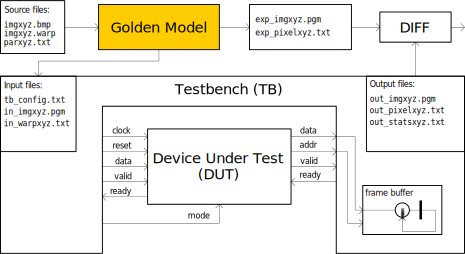
\includegraphics[width=\textwidth]{functional_verification_tb}
        \caption{Testbench used for functional verification.}%
        \label{fig:functional_verification_tb}
      \end{figure}

      Reference a ReadMe file that describes how the testbench can be launched.

    \subsubsection{Back-end implementation}

      In \gls{asic} projects, remember to discuss both front- and back-end implementation.
      That is, if you took special measures for floorplanning, \gls{dft}, or clock or power distribution, you will want to mention it here.
      In this case, make sure to add results that show the impact of your measures.

  \subsection{Results}

    Typical application-specific figures of merit of your hardware design are \gls{snr}, throughput, and memory/interface bandwidth.
    Moreover, you should also specify technology-specific figures such as area (for \glspl{asic}) or resource (for \glspl{fpga}) requirements, timing constraints, and power and energy consumption.

  \subsection{Data sheet}

    If your \gls{asic} is getting fabricated, you need to write a data sheet for it.
    You should put this data sheet into the appendix of your report.
    You are free to write the data sheet in a standalone document and include a \gls{pdf} file here or to write it in the source files of your report.

    Sections of a typical \gls{ic} data sheet are:
    \begin{itemize}
      \item Features
      \item Applications
      \item Packaging
      \item Bonding diagram like the one in \cref{fig:bonding_diagram}.
      \item Pinout diagram like the one in \cref{fig:asic_pinout}.
      \item Interface description
      \item Register map
      \item Operation modes:
      \begin{itemize}
        \item Functional modes
        \item Test modes
      \end{itemize}
      \item Electrical specifications
      \begin{itemize}
        \item Recommended operating regions
        \item Absolute maximum ratings
      \end{itemize}
    \end{itemize}

    \begin{figure}
      \centering
      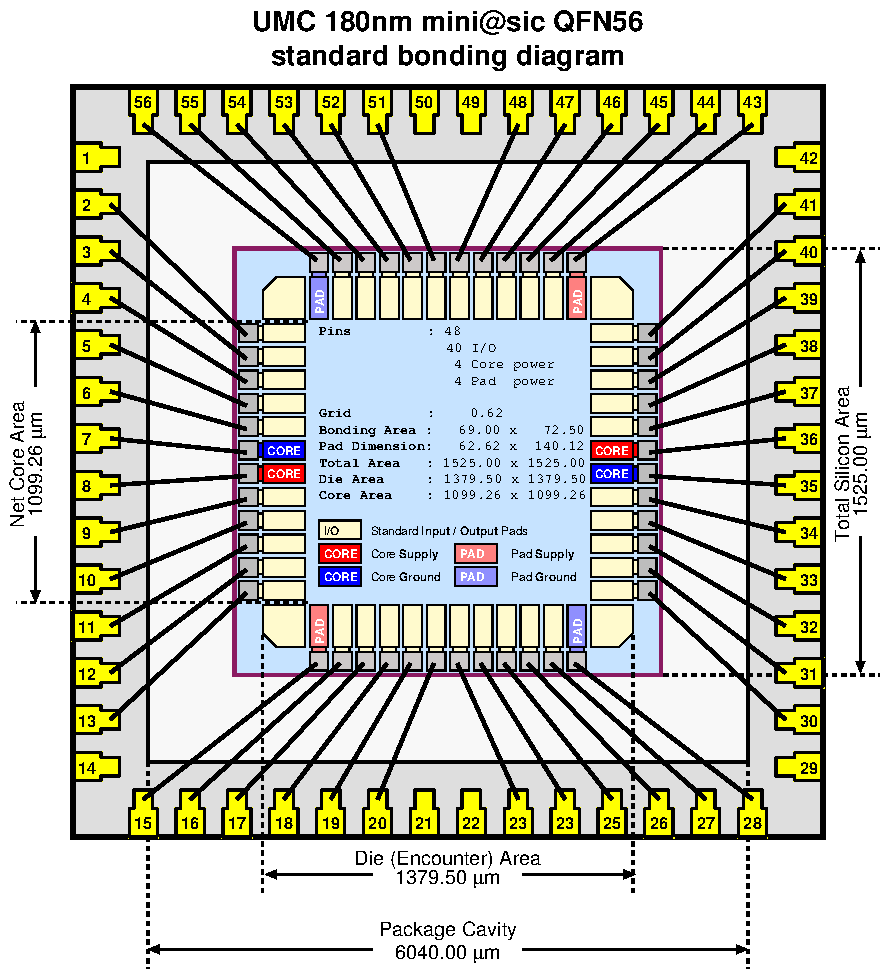
\includegraphics[width=.75\textwidth]{qfn56_180_std}
      \caption{Standard bonding diagram for QFN56 UMC 180\,nm mini@sics.}%
      \label{fig:bonding_diagram}
    \end{figure}

    \begin{figure}
      \centering
      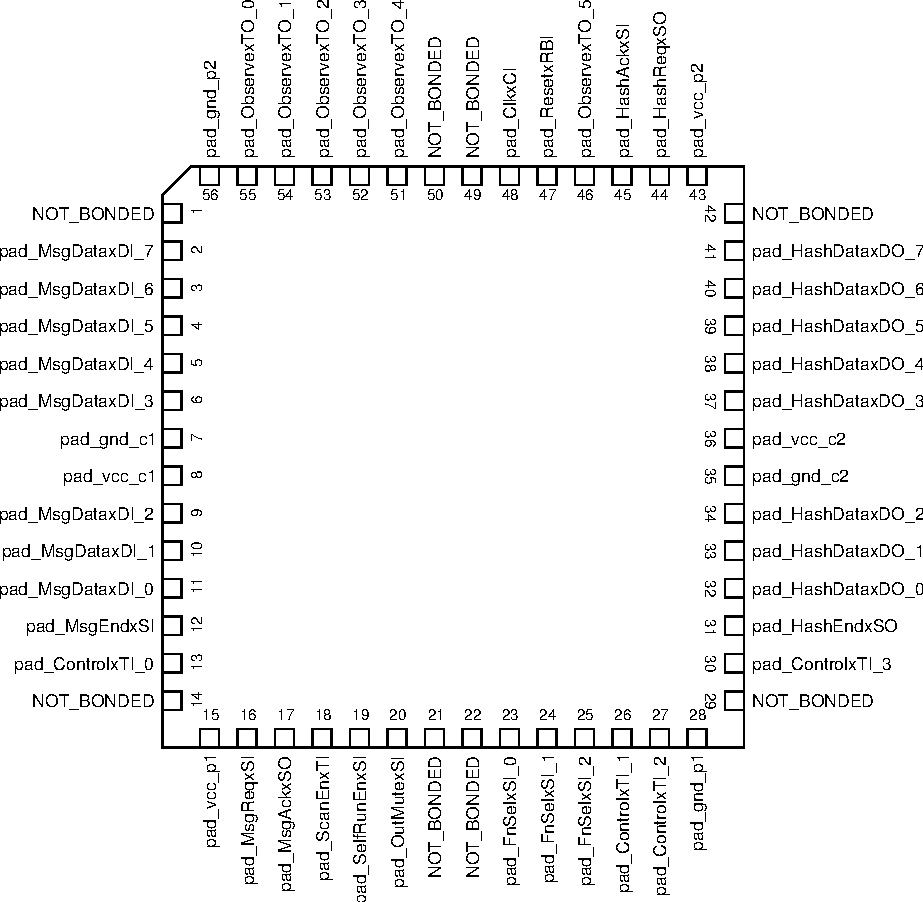
\includegraphics[width=.75\textwidth]{asic_pinout}
      \caption{Pinout for \textsc{MyFancyChip}.}%
      \label{fig:asic_pinout}
    \end{figure}

    For more information, up-to-date bonding diagrams, and other technology-specific data ask the \gls{dz}.
  % TODO: Remove these two appendices when you no longer need
%\chapter{Compact Guide to \LaTeX{} and the \textit{iisreport} Class}
\label{app:LaTeX_guide}

Writing a report with \LaTeX{} might at first not be as intuitive as with \gls{wysiwyg} editors.
However, once you get used to the (rather simple) syntax, you will soon discover how powerful it is and how it helps you achieve tasks that are very difficult (if not impossible) to achieve with \gls{wysiwyg} editors.

This report template provides everything you need to get you started working with \LaTeX{}.
The rest of this chapter contains a short guide with examples for commonly used features.

\section{Building the document}

  Generate a \gls{pdf} file from this template by simply executing \texttt{make} in the directory where the top-level \texttt{.tex} file is in.
  Internally, this will invoke the \texttt{latexmk} program, which is the simplest and most consistent way to build a \LaTeX{} document and is included in all recent \LaTeX{} distributions.
  Additionally, \texttt{make} will check the \texttt{fig/} directory and generate \gls{pdf} files for those figure raw files it knows how to compile (more on this in~\cref{sec:LaTeX_figures}).

\section{Text editing and spacing}

  White spaces and line breaks are automatically inserted when the document is compiled.
  For this, the number of spaces  between  two  words is irrelevant, but a different space length is automatically inserted after a period to make sentences better distinguishable.
  If you write a period that does not end a sentence, e.g., when mentioning Prof.\ Dr.\ S.\ Body, you need to escape the spaces between the abbreviated words with a backslash \verb|\|.
  If you want to prevent \LaTeX{} from breaking a line at a specific white space, you have to replace that space with a tilde \verb|~|.
  \LaTeX{} also automatically hyphenates English words, so it can break a line within a word, although it does so only cautiously.
  Automatic hyphenation can fail, e.g., for non-standard words, causing overly long lines.
  In such cases you have two options:
  First, if you have to break a standard word at an uncommon position, you can insert a \verb|\-| at that position in the word.
  Second, you can define the hyphenation of a non-standard word by adding \verb|\hyphenation{Jab-ber-woc-ky}| to the preamble\footnote{%
    The \emph{preamble} of a document is formed by all code between the \texttt{\textbackslash{}documentclass} command and the beginning of the document body after \texttt{\textbackslash{}begin\{document\}}.
  } of your document.

  A line of text is not broken at the same position as in the source code.
  For this reason, we suggest you put one sentence on one line of source code because this allows your \gls{vcs} to track content changes much better than if you wrap lines within sentences.
  To start a new paragraph, insert an empty line.
  You can manually break a line by writing \verb|\\|; however, this is rarely necessary and wide usage of it is a sign of fighting the typesetting system.

  By default in this template, paragraphs start with a short indentation and are not separated by vertical white space, but this can be changed.
  If you prefer the latter, pass the \texttt{parskip} option to the \texttt{iisreport} document class, i.e., change the first line of your main document to \verb|\documentclass[parskip]{iisreport}|.

  \subsection{Special characters}

    Many special characters are available, and they are all listed in \textsl{The Comprehensive \LaTeX{} Symbol List}~\cite{LaTeXSymbols}.
    At the beginning you might not know what to search for, though, so it can be more helpful to use the \textsl{Detexify}\footnote{\url{http://detexify.kirelabs.org/classify.html}} web app where you can draw the symbol you are looking for.

    A frequent mistake is to mix up the three dashes (-, --, and ---).
    The rules are simple~\cite{Knuth84}:
    \begin{itemize}
      \item The \emph{hyphen}, \verb|-|, is used between the elements of compound words; e.g., ``run-time''.
      \item The \emph{en-dash}, \verb|--|, is used for ranges; e.g., ``3--7''.
      \item The \emph{em-dash}, \verb|---|, is used for digressions within or at the end of a sentence---although you should use it sparingly.
    \end{itemize}

    Another frequent mistake are wrong quotation marks.
    Fortunately, this can also easily be avoided:
    Use \verb|`text'| for `single quotation marks' and \verb|``text''| for ``double quotation marks'' (have a look at the source code to see the matching pairs).
    In American English, double quotes prevail and single quotes are typically only used inside double quotes.

  \subsection{Font faces and emphasis}

    The font face can be changed locally with the commands in \cref{tbl:font_face_commands}.
    The text to appear differently has to be put between the curly braces \verb|{}|, i.e., the text is an \emph{argument} to one of the commands.
    Some font faces can also be combined by nesting them.
    For example, \verb|\textbf{\textit{some words}}| becomes \textbf{\textit{some words}}.

    \begin{table}
      \centerfloat
      \begin{tabular}{ l l }
        \toprule
        \textbf{Command} & \textbf{Output} \\
        \midrule
        \verb|\textrm{}| & \textrm{Roman (the default in this document)} \\
        \verb|\textsf{}| & \textsf{Sans serif} \\
        \verb|\texttt{}| & \texttt{Typewriter (i.e., all characters have the same width)} \\
        \verb|\textbf{}| & \textbf{Bold} \\
        \verb|\textit{}| & \textit{Italic} \\
        \verb|\textsl{}| & \textsl{Slanted} \\
        \verb|\textsc{}| & \textsc{Small caps} \\
        \bottomrule
      \end{tabular}
      \caption{Different font faces.}%
      \label{tbl:font_face_commands}
    \end{table}

    When you want to \emph{emphasize} text, use the \verb|\emph{}| command instead of one of the commands in \cref{tbl:font_face_commands}.
    In this way, you separate a \emph{property} of a piece of text (i.e., which text is emphasized) from its \emph{formatting} (i.e., how emphasized text looks like).
    This is an important principle in typesetting with \LaTeX{}.
    In this case, it allows you to define the formatting of all emphasized text independently of which text is meant to be emphasized.

  \subsection{Font sizes}

    The font size can be changed with the commands in \cref{tbl:font_sizes}.
    These commands change the size within a given \emph{scope}; for instance \verb|{\Large some words}| only prints ``some words'' large.

    \begin{table}
      \newcommand{\sampletext}{quick brown foxes}
      \centerfloat
      \begin{tabular}{ l l }
        \toprule
        \textbf{Command} & \textbf{Output sample} \\
        \midrule
        \verb|\tiny|          & {\tiny \sampletext} \\
        \verb|\scriptsize|    & {\scriptsize \sampletext} \\
        \verb|\footnotesize|  & {\footnotesize \sampletext} \\
        \verb|\small|         & {\small \sampletext} \\
        \verb|\normalsize|    & {\normalsize \sampletext} \\
        \verb|\large|         & {\large \sampletext} \\
        \verb|\Large|         & {\Large \sampletext} \\
        \verb|\LARGE|         & {\LARGE \sampletext} \\
        \verb|\huge|          & {\huge \sampletext} \\
        \verb|\Huge|          & {\Huge \sampletext} \\
        \bottomrule
      \end{tabular}
      \caption{Different font sizes.}%
      \label{tbl:font_sizes}
    \end{table}

  \subsection{Coloring text}

    \begin{figure}
      \centerfloat
      \begin{minipage}{1.1\textwidth}
        % Source: colors from `xcolor`, sorting by own implementation.
        \def\0#1{\colorbox{#1}{\phantom{XX}}~#1\\}
        \scriptsize
        \begin{multicols}{5}
          \noindent
          \0{Magenta}
          \0{Rhodamine}
          \0{VioletRed}
          \0{CarnationPink}
          \0{Lavender}
          \0{RubineRed}
          \0{WildStrawberry}
          \0{OrangeRed}
          \0{Salmon}
          \0{Maroon}
          \0{Red}
          \0{Mahogany}
          \0{BrickRed}
          \0{Melon}
          \0{RedOrange}
          \0{Sepia}
          \0{Brown}
          \0{Bittersweet}
          \0{RawSienna}
          \0{Peach}
          \0{Orange}
          \0{Tan}
          \0{Apricot}
          \0{BurntOrange}
          \0{YellowOrange}
          \0{Dandelion}
          \0{Goldenrod}
          \0{Yellow}
          \0{GreenYellow}
          \0{SpringGreen}
          \0{LimeGreen}
          \0{YellowGreen}
          \0{OliveGreen}
          \0{Green}
          \0{ForestGreen}
          \0{SeaGreen}
          \0{PineGreen}
          \0{JungleGreen}
          \0{Emerald}
          \0{TealBlue}
          \0{BlueGreen}
          \0{Aquamarine}
          \0{Turquoise}
          \0{SkyBlue}
          \0{Cyan}
          \0{ProcessBlue}
          \0{Cerulean}
          \0{MidnightBlue}
          \0{CornflowerBlue}
          \0{RoyalBlue}
          \0{NavyBlue}
          \0{CadetBlue}
          \0{Periwinkle}
          \0{Blue}
          \0{BlueViolet}
          \0{Violet}
          \0{RoyalPurple}
          \0{Purple}
          \0{Fuchsia}
          \0{Plum}
          \0{Orchid}
          \0{Mulberry}
          \0{DarkOrchid}
          \0{Thistle}
          \0{RedViolet}
        \end{multicols}
        \begin{multicols}{5}
          \noindent
          \columnbreak
          \0{black}
          \0{darkgray}
          \0{gray}
          \0{lightgray}
          \0{white}
        \end{multicols}
      \end{minipage}
      \caption{Selected predefined colors, sorted by hue.}%
      \label{fig:selected_colors}
    \end{figure}

    The color of text can be changed with the \verb|\textcolor| and \verb|\color| commands:
    The former takes two arguments, a declared color and the text to color.
    For example, \verb|\textcolor{RoyalBlue}{I am royal}| becomes \textcolor{RoyalBlue}{I am royal}.
    The latter takes only a defined color and colors all text in its scope.
    For example, \verb|{\color{RoyalPurple}So am I}| becomes {\color{RoyalPurple}So am I}.

    \Cref{fig:selected_colors} shows a selection of predefined colors.
    The \texttt{xcolor} package manual~\cite{xcolor} lists more colors and describes how to define custom colors.

\section{Debugging}

  Occasionally, you will make syntax mistakes while writing a document, causing compilation to fail.
  In this case, the last lines of the console output will mention an error and point you to a \texttt{.log} file in the directory where you ran \texttt{make}.
  Open that log file.
  Even though that file can be very long and contains many technical details that are of no interest to you, finding errors is easy: simply search for lines starting with an exclamation mark!

  If you use an undefined command, e.g., due to a typo, the error messages should be very helpful.
  If, however, you cause parentheses or environment delimiters to mismatch, the position of your mistake is hard to derive from the error messages.

  A good technique to locate a mistake is to comment out recent changes until the document compiles neatly again.
  For recompilation, you should use \texttt{make clean all} to prevent errors that crept into temporary files from disturbing your bug hunt.
  To reduce compilation time for large documents, you can comment out chapters that are known to be good.
  When you have a working version again, re-enable the code you commented out last piece-by-piece.
  This piecewise reduction should help you systematically find the mistake.

\section{Math mode}

  \LaTeX{} is probably the most powerful and elaborate tool to typeset mathematical content.
  Once you know a few core concepts, writing properly formatted mathematical content becomes quite simple.

  To distinguish maths from regular text, maths is written in \emph{math mode}.
  There are two categories that differ in their presentation: inline and displayed.
  Inline maths, e.g., $ a\sp{2} + b\sp{2} = c\sp{2} $ is enclosed in \verb|$| signs.
  It is meant for simple expressions.
  More complex content is displayed separately from the text.
  The most common way to display maths is inside the \texttt{equation} environment\footnote{%
    \emph{Environments} in \LaTeX{} are similar to commands, but are usually used for larger chunks of code.
    For example, the entire document except the preamble is inside the \texttt{document} environment.
    Environments are formed with \texttt{\textbackslash{}begin\{environmentname\}} \texttt{...} \texttt{\textbackslash{}end\{environmentname\}}.
  }, for example:
  \begin{equation}
    \int\sb{-\infty}\sp{\infty} x \dif x = 0.
  \end{equation}

  Subscripts are written with \verb|\sb{}|\footnote{%
    By default, \LaTeX{} would allow to use the underscore \texttt{_} for subscripts.
    In the \texttt{iisreport} document class, however, the underscore is a regular, printable character.
    The rationale is that the underscore is very common in technical designators and having to escape every single one is a common source of errors.
  }, superscripts with \verb|\sp{}|, integrals with \verb|\int|, and sums with \verb|\sum|.
  Have a look at the source code of the last paragraph for usage examples.

  Equations get a number by default, so you can label and refer to them (more on this in \cref{sec:cite_and_reference}).
  If you want to suppress an equation number, you can use the \emph{starred} version of the equation environment, i.e., \verb|equation*|.

  Many mathematical symbols and functions are predefined, letting you express relations such as $ \forall x \in \mathbb{R} $ $ \exists n \in \mathbb{N}: \ldots $ fluently.
  Wikipedia\footnote{\url{https://en.wikibooks.org/wiki/LaTeX/Mathematics\#List_of_Mathematical_Symbols}} has a list of all predefined mathematical symbols.

  Variable names are by default one character long, causing \verb|$ xy z $| to be typeset with identical spacing as \verb|$ xyz $|.
  You should thus use single-letter variables whenever possible.
  If you have to use multi-letter variables, write them inside the \verb|\var{}| command\footnote{%
    The \texttt{var} command is not standard \LaTeX{} but defined by the \texttt{iisreport} document class.
    If you want to use it elsewhere, it is very simple to implement: \url{https://tex.stackexchange.com/a/129434/92384}.
  }.
  This causes $ x $ and $ y $ in the two-letter variable $ \var{xy} $ to be closer together.
  To make the variable clearly distinguishable from the next one, however, you may still have to insert a space\footnote{%
    The most common horizontal spacing macros in math mode are (in increasing order):
    \texttt{\textbackslash{},}, \texttt{\textbackslash{};}, \texttt{\textbackslash{}enspace}, \texttt{\textbackslash{}quad}, and \texttt{\textbackslash{}qquad}.
    A complete list with examples is available here: \url{https://tex.stackexchange.com/a/74354/92384}.
    Keep in mind that frequent insertion of manual spacing may be a hack around a more fundamental problem.
  } (as in $ \var{xy} \, z $) or even an operator (as in $ \var{xy} \cdot z $).

  When you want to use text in math mode (subscripts are a common use case for this), you must write that text inside the \verb|\text{}| command to avoid the same problems as with multi-letter variables.

  \subsection{Delimiters: Parentheses, brackets, bars, and intervals}

    For simple parentheses and square brackets, you can readily use the \texttt{()} and \texttt{[]} characters, respectively.
    Curly braces are a bit more involved because \verb|{}| are grouping characters.
    Thus, you would have to escape them and write \verb|\{\}| instead.
    However, we recommend to use the \verb|\cbr{}| command (short for ``curly braces'') instead.
    That command has the additional advantage of automatically sizing parentheses to the content.
    (The automatic sizing can be disabled by passing \verb|[0]| as optional first argument to the command.)
    If you need automatically sized parentheses and square brackets, the commands are \verb|\del{}| (for ``delimiter'') and \verb|\sbr{}| (for ``square bracket''), respectively.
    This allows you to effortlessly maintain readability even in deeply nested equations:
    \begin{equation}
      \del{E\sbr{\min\cbr{X\sb{1}, X\sb{2}}} - \del{\pi - \arccos\del{\frac{y}{r}}}}\sp{n}.
    \end{equation}

    Absolute values are written with \verb|\abs{}|, e.g.,
    \begin{equation}
      \abs{\exp\del{x \pi i}} = 1 \quad\forall x \in \mathbb{R},
    \end{equation}
    while vector norms are written with \verb|\norm{}|, e.g.,
    \begin{equation}
      \norm{\vec{x}}\sb{2} = \sqrt{\sum\sb{k=1}\sp{n} x\sb{k}\sp{2}} \quad\forall \vec{x} \in \mathbb{R}\sp{n},
    \end{equation}
    where the vector $ \vec{x} $ was written with \verb|\vec{x}| and the square root with \verb|sqrt{..}|.

    Intervals are written with the \verb|\intxy{}| commands, where each of \texttt{x} and \texttt{y} are either \texttt{o} for open or \texttt{c} for closed.

  \subsection{Differential and derivative operators}

    Differential and derivative operators are written with the following commands:
    \verb|\dif x| is the simple differential operator, e.g., $ \dif x $.
    \verb|\Dif x| is a derivative operator, e.g., $ \Dif x $.
    \verb|\od[n]{f}{x}| is the ordinary $n$-th derivative operator, e.g., $ \od[n]{f}{x} $.
    \texttt{n} is optional and should be omitted for the first derivative.
    \verb|\pd[n]{f}{x}| is the partial $n$-th derivative operator, e.g., $ \pd[n]{f}{x} $.
    Finally, \verb|\md{f}{n}{x}{q}{y}{r}| is the mixed partial derivative operator, e.g., $ \md{f}{n}{x}{q}{y}{r} $, where \texttt{n} is the total order of differentiation and \texttt{q} and \texttt{r} are the orders of differentiation for \texttt{x} and \texttt{y}, respectively.

  \subsection{Vectors, matrices, and distinction of cases}

    Both vectors and matrices are written with the \texttt{Xmatrix} environments, where \texttt{X} defines the delimiter of the matrix and can be \texttt{p} for parentheses, \texttt{b} for brackets, \texttt{B} for curly braces, \texttt{v} for vertical bars, \texttt{V} for double vertical bars, or omitted for no delimiters.
    The matrix is written row-wise with the elements of a row separated by \verb|&| and each row is terminated by \verb|\\|.
    A column vector is just a matrix with one column, a row vector one with one row.
    For example:
    \begin{equation}
      x = \begin{pmatrix}
        x\sb{1} & x\sb{2} \\
      \end{pmatrix}
      \quad
      y = \begin{pmatrix}
        y\sb{1} \\
        y\sb{2} \\
      \end{pmatrix}
      \quad
      A = \begin{pmatrix}
        a\sb{1,1} & a\sb{1,2} \\
        a\sb{2,1} & a\sb{2,2} \\
      \end{pmatrix}
    \end{equation}

    The \texttt{Xmatrix} environments center the columns by default.
    If you want a different alignment, use the starred variant\footnote{%
      The \emph{starred variant} of an environment or a command simply has a star \texttt{*} at the end of the environment or command name, respectively.
      Not all environments and commands have a starred variant.
    } of the environments, which accepts a single character as optional argument\footnote{%
      \emph{Optional arguments} are always enclosed in square brackets \texttt{[]}.
    }: \texttt{r} for right, \texttt{c} for center, and \texttt{l} for left.

    To write case distinctions, use the \texttt{dcases} environment.
    For example:
    \begin{equation}
      a(v) =
      \begin{dcases}
        0             & \text{if } v \geq \mathrm{c}, \\
        \epsilon > 0  & \text{else}.
      \end{dcases}
    \end{equation}
    If you want the curly brace to be on the right of the cases, use the \texttt{rcases} environment.

  \subsection{Multi-line equations}

    If you want to write a single equation that is longer than one line, use the \texttt{multline} (without `i'!) environment.
    That environment switches to math mode by itself, so you \emph{must not} use it inside \texttt{equation}.
    Use the line break command, \verb|\\|, to define the two lines of the equation.
    For example:
    \begin{multline}
      \alpha + \beta + \gamma + \delta + \epsilon + \zeta + \eta + \theta + \iota + \kappa + \lambda + \mu + \nu + \xi + + \pi + \rho + \sigma + \tau \\
       = \upsilon + \phi + \chi + \psi + \omega.
    \end{multline}

    To write multiple equations in series or an especially complicated multi-line equation, use the \texttt{IEEEeqnarray} environment.
    That environment takes a series of characters specifying the columns as argument.
    The most common argument is \texttt{rCl}, meaning one right-aligned column followed by a center-aligned separator followed by a left-aligned column.
    As with matrices, use \verb|&| to separate columns and \verb|\\| to separate equation lines.
    For example:
    \begin{IEEEeqnarray}{rCl}
      a & = & b + c \\
        & = & d + e + f + g + h + i + j + k \nonumber\\
        &   & +\> l + m + n + o \\
        & = & p + q + r + s,
    \end{IEEEeqnarray}
    where the first line of the second equation was ended by \verb|\nonumber| to suppress numbering that part of the equation.

    Browse through \textsl{How to Typeset Equations in \LaTeX{}}~\cite{LaTeXEquations} for further informations and solutions to more complex examples.

  \subsection{Definitions, theorems, lemmas, and proofs}

    Here are some examples on writing definitions, theorems, lemmas, and proofs.

    \begin{definition}[Singularity]
      Let $ U $ be an open subset of the complex numbers $ \mathbb{C} $, $ a \in U $, and $ f $ be a complex differentiable function defined on $ U \setminus \cbr{a} $.

      The point $ a $ is a \emph{removable singularity} of $ f $ if there exists a holomorphic function $ g $ defined on all of $ U $ such that $ f(z) = g(z) \>\forall z \in U \setminus \cbr{a} $.

      The point $ a $ is a \emph{pole} or \emph{non-essential singularity} of $ f $ if there exists a holomorphic function $ g $ defined on $ U $ with $ g(a) \neq 0 $ and $ n \in \mathbb{N} $ such that
      \begin{equation}
         f(z) = \frac{g(z)}{(z - a)\sp{n}} \quad\forall z \in U \setminus \cbr{a}.
      \end{equation}
      The lowest such number $ n $ is called the \emph{order of the pole}.

      The point $ a $ is an \emph{essential singularity} of $ f $ if it is neither a removable singularity nor a pole.
      The point $ a $ is an essential singularity iff the Laurent series has infinitely many powers of negative degree.
    \end{definition}

    \begin{theorem}[Residue Theorem]
      Let $ f $ be analytic in the region $ G $ except for the isolated singularities $ a\sb{1} $, $ a\sb{2} $, \ldots, $ a\sb{m} $.
      If $ \gamma $ is a closed rectifiable curve in $ G $ that does not pass through any of the points $ a\sb{k} $ and if $ \gamma \approx 0 $ in $ G $, then
      \begin{equation}
        \frac{1}{2 \pi i} \int\sb{\gamma} f = \sum\sb{k = 1}\sp{m} n(\gamma; a\sb{k}) \,\text{Res}(f; a\sb{k}).
      \end{equation}
    \end{theorem}

    \begin{proof}
      Left as an exercise for the reader.
    \end{proof}

    \begin{lemma}[Schwarz]
      Let $ D \coloneqq \cbr{z \in \mathbb{C}: \abs{z} < 1} $ be the open unit disk in the complex plane centered at the origin, and let $ f: D \to \mathbb{C} $ be a holomorphic map such that $ f(0) = 0 $ and $ \abs{f(z)} \leq 1 $ on $ D $.
      Then, $ \abs{f(z)} \leq \abs{z} \>\forall z \in D $ and $ \abs{f'(0)} \leq 1 $.
      Moreover, if $ \abs{f(z)} = \abs{z} $ for some $ z \neq 0 $ or $ \abs{f'(0)} = 1 $, then $ f(z) = a z $ for some $ a \in \mathbb{C} $ with $ \abs{a} = 1 $.
    \end{lemma}

    \begin{proof}
      Beyond the scope of this document.
    \end{proof}

\section{Quantities with SI units}

  \begin{itemize}
    \item quantity with a unit: \SI{300}{\mega\hertz}
    \item unit alone: \si{\giga\volt}
    \item ranges of quantities with units: \SIrange{2}{256}{\mebi\bit\per\second}
    \item number (especially for engineering notation or very large numbers): \num{10000}, \num{3.14e6}, \num{5e-12}
    \item ranges of numbers \numrange{5e-12}{3.14e6}
  \end{itemize}

  Math mode not required, but can be used with it.

\section{Enumerations and itemizations}

  Itemizations are \ldots
  \begin{itemize}
    \item unnumbered and
    \item written inside the \texttt{itemize} environment, where every item starts with \verb|\item|.
  \end{itemize}

  Enumerations, on the other hand, are \ldots
  \begin{enumerate}
    \item numbered and
    \item written inside the \texttt{enumerate} environment.
  \end{enumerate}

  Both itemizations and enumerations can be nested.
  The indentation level and itemization items are then automatically adjusted:
  \begin{enumerate}
    \item This demonstrates that
    \begin{enumerate}
      \item enumerations and
      \item itemizations
      \begin{itemize}
        \item can be nested.
      \end{itemize}
    \end{enumerate}
  \end{enumerate}

\section{Floats: figures and tables}
\label{sec:LaTeX_figures}

  Both figures and tables normally form \emph{floating} environments.
  This means that \LaTeX{} will automatically place them near to where they were in the source code, but not at the exact same position.
  The placement algorithm is fairly sophisticated~\cite{LaTeXFloatPlacement} and usually works reasonably well.

  The base environment for figures is \texttt{figure}, the one for tables is \texttt{table}.
  Floats usually get a caption with the \verb|\caption{}| command.
  If you want to refer to them (more on this in \cref{sec:cite_and_reference}), you additionally have to put a \verb|\label{}| after the \verb|\caption{}| but on the same line (to have correct page numbers even near page breaks).

  To center-align the content of a float, use the \verb|\centerfloat| command at the beginning of that float.

  \subsection{Figures}

    Images can be included with the \verb|\includegraphics[properties]{file_name}| command, where \texttt{properties} allows to, e.g., define the \texttt{width}, \texttt{height}, or \texttt{scale} of an image in the \texttt{key=value} syntax.
    The \texttt{file_name} is relative to the \texttt{fig/} directory and the default suffix, \texttt{.pdf}, can be omitted.
    An example figure is given in \cref{fig:example_figure}.

    \begin{figure}
      \centerfloat
      
\includegraphics[width=5cm]{eth_logo}
      % Note: We do not have the SVG source file for the image above, so we have to put the PDF under version control.
      \caption{Example figure.}%
      \label{fig:example_figure}
      % Note: The `\label{}` can be on the line after the `\caption{}` if the `\caption{}` line ends with a comment.
    \end{figure}

    Whenever possible, you should use \glspl{svg} for two reasons:
    First, they can be scaled losslessly to the target size and resolution.
    Second, they allow you to keep a small, modifiable source file of the graphic under version control and have the \gls{pdf} file to be included built automatically.

    We recommend using \textsl{Inkscape}\footnote{Freely available at \url{https://inkscape.org}.}.
    Simply draw a figure in Inkscape, set the canvas to where you want the image border, save the original \texttt{.svg} file in the \texttt{fig/} directory, and use \verb|\includegraphics| on the file name without suffix.
    When you run \texttt{make}, the corresponding \gls{pdf} file will get built automatically and included in your document.
    If you use a \gls{vcs} (we highly recommend to do so!), track the original \texttt{.svg} file but add the auto-built \texttt{.pdf} file to the ignore list (e.g., \texttt{fig/.gitignore}).
    If you include \gls{pdf} files of which you have no source files, track that \texttt{.pdf} file in your \gls{vcs}.

    As Inkscape does not support embedding fonts in its \gls{svg} files, you should either only use standard, widely-available fonts\footnote{\href{https://www.w3schools.com/cssref/css_websafe_fonts.asp}{Web safe fonts} are good candidates for widely available fonts.} or track the auto-built \gls{pdf} images in \texttt{fig/} with your \gls{vcs}.
    If you choose the latter, though, be aware that other collaborators who do not have the font installed must not commit changes to the built \gls{pdf} images (because text with missing fonts will be rendered incorrectly by their Inkscape).

  \subsection{Tables}

    \begin{table}
      \centerfloat
      \begin{tabular}{ r r r r }
        \toprule
        \textbf{Decimal} & \textbf{Hexadecimal} & \textbf{Octal} & \textbf{Binary} \\
        \midrule
        10 & $ \mathtt{A}\sb{16} $ & $ \mathtt{12}\sb{8} $ & $ \mathtt{1010}\sb{2} $ \\
        13 & $ \mathtt{D}\sb{16} $ & $ \mathtt{15}\sb{8} $ & $ \mathtt{1101}\sb{2} $ \\
        \bottomrule
      \end{tabular}
      \caption{Simple example table with some values in different number systems.}%
      \label{tbl:sample_number_systems}
    \end{table}

    \begin{table}
      \centerfloat
      \rowcolors{2}{lightgray}{white}
      \begin{tabular}{ c c c }
        \toprule
        \textbf{Some} & \textbf{title} & \textbf{words} \\
        \midrule
        odd   & odd & odd \\
        even  & \cellcolor{darkgray}\color{white} even  & even  \\
        odd   & odd & odd \\
        \bottomrule
      \end{tabular}
      \caption{Simple example table with different row and cell colors.}%
      \label{tbl:sample_colors}
    \end{table}

    \begin{table}
      \centerfloat
      \begin{tabular}{ l p{1.5cm} p{1.5cm} p{7cm} }
        \toprule
        \textbf{Day} & \textbf{Min.\ Temp.} & \textbf{Max.\ Temp.} & \textbf{Description} \\
        \midrule
        Monday  & \SI{11}{\degreeCelsius} & \SI{22}{\degreeCelsius} & A clear day with lots of sunshine. However, a strong breeze will bring down the temperatures. \\
        Tuesday & \SI{9}{\degreeCelsius}  & \SI{19}{\degreeCelsius} & Cloudy with rain across many northern regions.  Clear spells across most of Scotland and Northern Ireland, but rain reaching the far northwest. \\
        \bottomrule
      \end{tabular}
      \caption{%
        Example table with fixed column widths: \SI{1.5}{\centi\meter} for columns two and three, \SI{7}{\centi\meter} for column four.
        Content adopted from \href{https://en.wikibooks.org/wiki/LaTeX/Tables\#Text_wrapping_in_tables}{Wikibooks}.
      }%
      \label{tbl:fixed_width_columns}
    \end{table}

\section{Algorithms and source code listings}

  \Cref{alg:disjoint_decomposition} shows an example algorithm.
  Have a look at the source code to discover how it works.

  \begin{algorithm}
    \SetKwData{Left}{left}\SetKwData{This}{this}\SetKwData{Up}{up}
    \SetKwFunction{Union}{Union}\SetKwFunction{FindCompress}{FindCompress}
    \SetKwInOut{Input}{input}\SetKwInOut{Output}{output}

    \Input{A bitmap $Im$ of size $w\times l$}
    \Output{A partition of the bitmap}
    \BlankLine
    \emph{special treatment of the first line}\;
    \For{$i\leftarrow 2$ \KwTo $l$}{
      \emph{special treatment of the first element of line $i$}\;
      \For{$j\leftarrow 2$ \KwTo $w$}{\label{forins}
        \Left$\leftarrow$ \FindCompress{$Im[i,j-1]$}\;
        \Up$\leftarrow$ \FindCompress{$Im[i-1,]$}\;
        \This$\leftarrow$ \FindCompress{$Im[i,j]$}\;
        \If(\tcp*[h]{O(\Left,\This)==1}){\Left compatible with \This}{\label{lt}
          \lIf{\Left $<$ \This}{\Union{\Left,\This}}
          \lElse{\Union{\This,\Left}}
        }
        \If(\tcp*[f]{O(\Up,\This)==1}){\Up compatible with \This}{\label{ut}
          \lIf{\Up $<$ \This}{\Union{\Up,\This}}
          \tcp{\This is put under \Up to keep tree as flat as possible}\label{cmt}
          \lElse{\Union{\This,\Up}}\tcp*[r]{\This linked to \Up}\label{lelse}
        }
      }
      \lForEach{element $e$ of the line $i$}{\FindCompress{p}}
    }
    \caption{Disjoint decomposition.}%
    \label{alg:disjoint_decomposition}
  \end{algorithm}

  Source code listings are written inside the \texttt{lstlisting} environment, which takes optional arguments such as the \texttt{language} of the code, a \texttt{caption}, and a \texttt{label} in \verb|key=value| syntax.
  \Cref{lst:simple_C} shows an example listing.

  \begin{lstlisting}[language=C, caption={Simple C code snippet.}, label={lst:simple_C}]
    int main()
    {
      return 0;
    }
  \end{lstlisting}

  External source code files can be included as listing with the \verb|\lstinputlisting{}| command.
  Since you rarely want to include an entire file, you can specify the first and the last line with the \texttt{firstline} and the \texttt{lastline} key, respectively.

\section{Citing and referencing}
\label{sec:cite_and_reference}

  Use the \verb|\cref{}| command to reference a document-internal label.
  Use the \verb|\cite{}| command to cite an entry in the bibliography.
  You should always use a nonbreaking space, \verb|~|, before the \verb|\cite{}| command to prevent the citation label from falling to the next line.

\section{Printing and binding}

  When printing this document, pass the \texttt{print} option to the \texttt{iisreport} class.
  This will cause the layout to be optimized for printing.

\section{Further reading}

  For a guide on writing research reports, we recommend the \textsl{Manual for Writers of Research Papers, Theses, and Dissertations}~\cite{Turabian13}.
  Furthermore, \textsl{The Elements of Style}~\cite{Strunk12} and \textsl{The Chicago Manual of Style}~\cite{ChicagoManualOfStyle} are useful guides on concise writing in general.
  The latter is freely available online within the ETH network.\footnote{\url{http://www.chicagomanualofstyle.org}}

  If you are interested to learn more about \LaTeX{}, you will find many resources online but the majority of them are written by casual amateurs and can teach you bad practices.
  Their approach is not strictly wrong but in the long term can cost you a lot of time compared to proper solutions.
  Thus, let us suggest to start all your \TeX{}-related searches at the \TeX{} StackExchange\footnote{\url{https://tex.stackexchange.com/}} community.
  Especially in the beginning, you will encounter common problems, for which there are usually several high-quality solutions on StackExchange, complete with an explanation of why the problem arose.

  There are also some very good books on \LaTeX{}.
  \textsl{The Not So Short Introduction to \LaTeX2e{}}~\cite{LaTeXIntroduction} is an excellent start, and \textsl{More Math into \LaTeX{}}~\cite{Graetzer16} teaches \SI{99}{\percent} of what you need to know about typesetting maths.
  The first book\footnote{\url{http://tobi.oetiker.ch/lshort/lshort.pdf}} and the first section of the second book\footnote{\url{http://www.ctan.org/tex-archive/info/Math_into_LaTeX-4/Short_Course.pdf}} are freely available online.
  For more advanced users, \textsl{The \LaTeX{} Companion}~\cite{Mittelbach04} and the \textsl{The \TeX{}book}~\cite{Knuth84} are the definitive books.

\section{\textit{iisreport} options quick reference}

  The \textit{iisreport} document class offers a few options that allow you to easily customize the layout of your report and configure certain features.
  Options can be specified inside the square brackets on the first line of the \texttt{report.tex} file, with individual options separated by commas.
  Here is an overview of all available options in alphabetic order:

  \begin{itemize}[itemsep=0pt]
    \item \texttt{oldfonts} brings back the fonts from the legacy \acrshort{iis} report template.
    \item \texttt{oldsubscript} disables making the underscore printable and makes it usable for subscripts instead.
    \item \texttt{parskip} causes paragraphs to start with a vertical space of half a line instead of indentation.
    \item \texttt{print} optimizes the page layout for printing and binding.
  \end{itemize}
          % their guidelines.
\chapter{Task Description}

\sloppypar

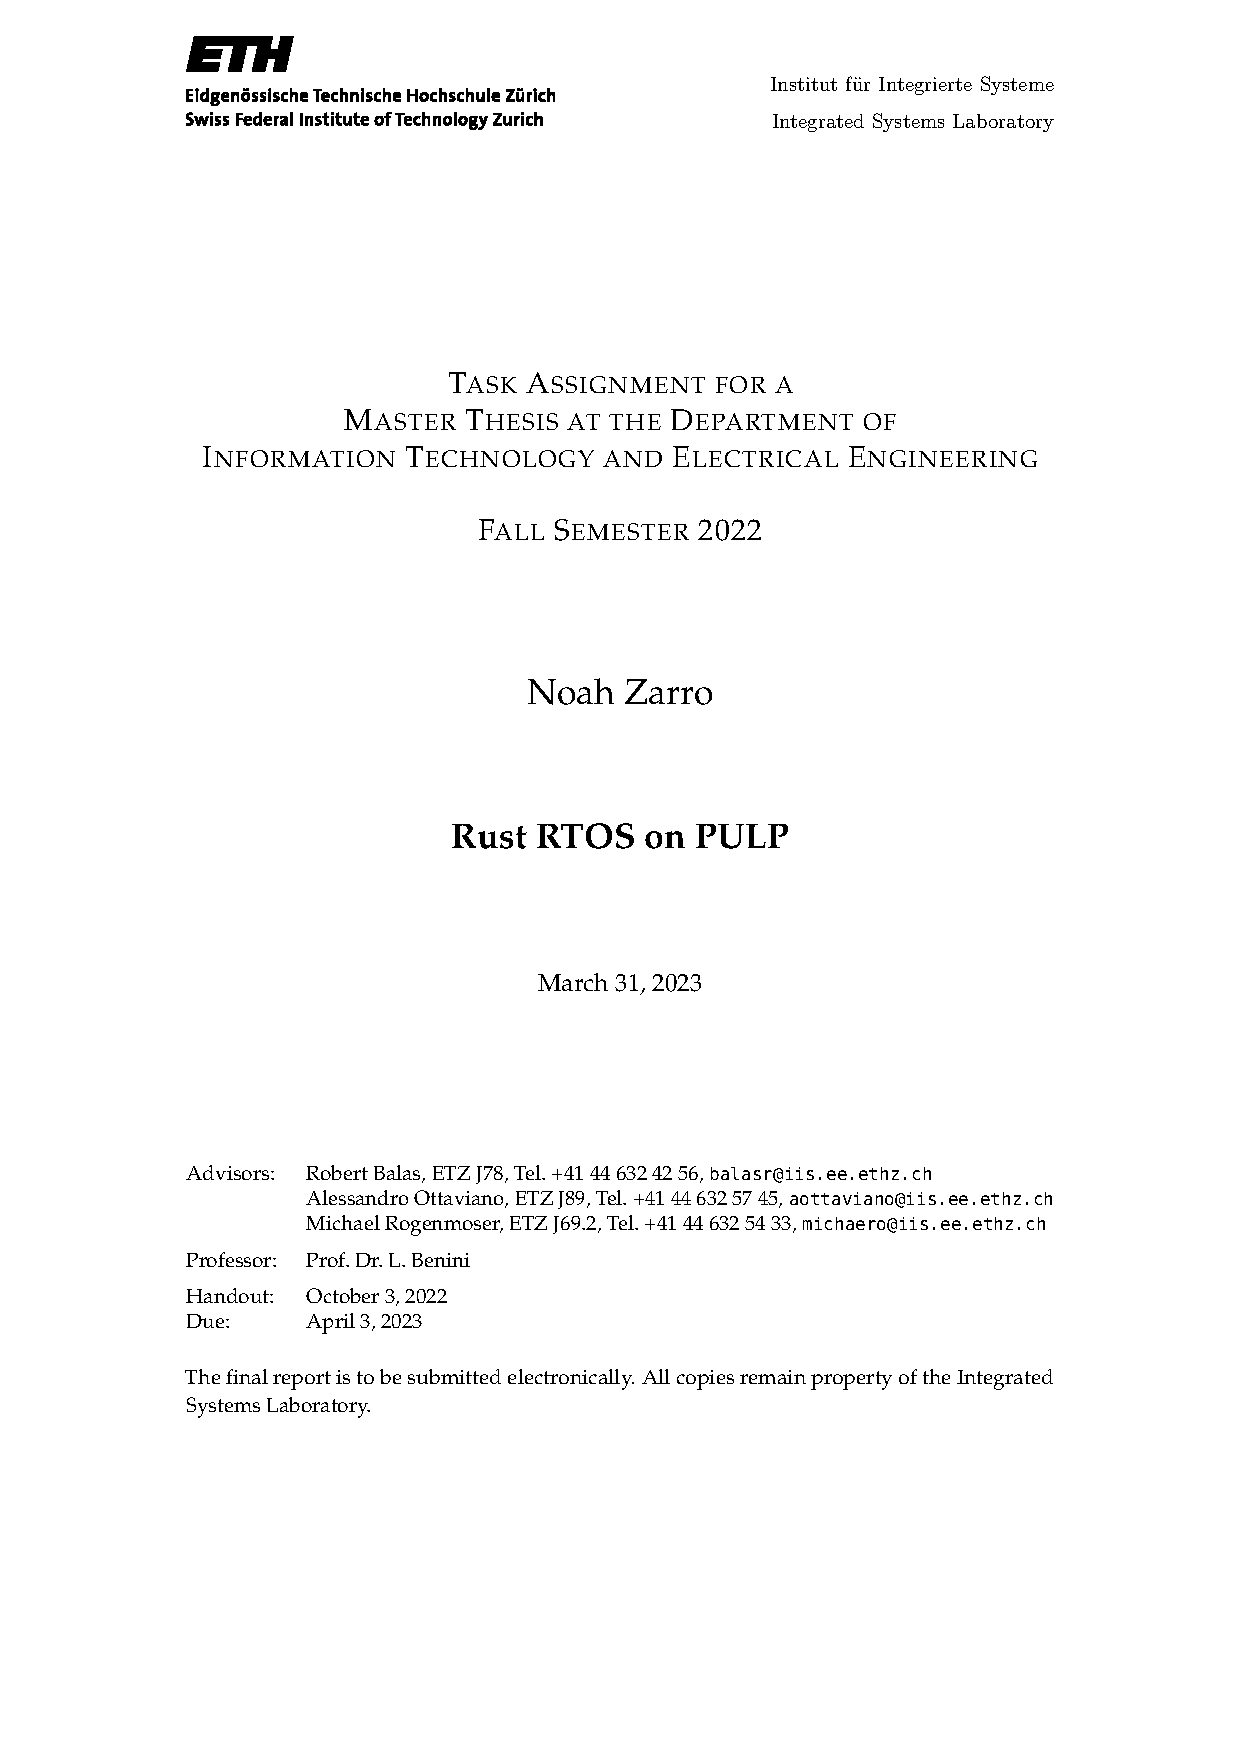
\includepdf[pages=-, scale=0.9]{Noah_Zarro_Task_Description_v1.pdf}

\backmatter

% Format: \newacronym{handle}{acronym}{full term}
% The full term should be in title case for proper names and in sentence case otherwise.
% If in doubt about hyphenation or case style, refer to the English Wikipedia.
\newacronym{rtos}{RTOS}{Real-time operating system}
\newacronym{rtic}{RTIC}{Real-Time Interrupt-driven Concurrency}
\newacronym{iis}{IIS}{Integrated Systems Laboratory}
\newacronym{hal}{HAL}{Hardware Abstraction Layer}
\newacronym{pulp}{PULP}{Parallel Ultra Low Power}
\newacronym{mac}{MAC}{Micro-architecture Crate}
\newacronym{pac}{PAC}{Periperal Access Crate}
\newacronym{clic}{CLIC}{Core-Local Interrupt Controller}
\newacronym{nvic}{NVIC}{Nested Vectored Interrupt Controller}
\newacronym{csr}{CSR}{Control Status Register}
\newacronym{soc}{SoC}{System on a Chip}
\newacronym{pdf}{PDF}{Portable Document Format}
\newacronym{spse}{SPSE}{Situation-Problem-Solution-Evaluation}
\newacronym{svg}{SVG}{scalable vector graphics}
\newacronym{vcs}{VCS}{version control system}
\newacronym{wysiwyg}{WYSIWYG}{``what you see is what you get''}

 % TODO: Remove this line when you no longer need the writing guidelines.
\listofacronyms

\listoffigures
\listoftables

 % TODO: Remove the `latex_and_writing` bibliography when you no longer need that guide.
\bibliography{./bib/main,./bib/latex_and_writing}

\end{document}
